\documentclass[11pt,a4paper]{article}
\usepackage[utf8]{inputenc}
\usepackage{amsmath}
\usepackage{amsfonts}
\usepackage{amssymb}
\usepackage{ngerman}
\usepackage{graphicx}
\usepackage{geometry}
\usepackage{setspace}
\usepackage{cite}
\usepackage{url}
\usepackage{caption}
\usepackage{tikz}
\usepackage{colortbl}
\usepackage{sidecap}
\usepackage{wrapfig}
\usepackage[T1]{fontenc}
\usepackage{listings}
\usetikzlibrary{decorations.pathreplacing}

\overfullrule=0pt

\definecolor{code_comment}{RGB}{180, 180, 180}
\definecolor{code_keyword}{RGB}{0, 200, 00}
\definecolor{code_background}{RGB}{40, 40, 40}
\definecolor{dark_red}{RGB}{230, 40, 40}

\lstset{
  backgroundcolor=\color{code_background},
  basicstyle=\small\ttfamily\color{white},
  keywordstyle=\bfseries\ttfamily\color{code_keyword},
  stringstyle=\color{red}\ttfamily,
  commentstyle=\color{code_comment}\ttfamily,
  emph={comment},
  showstringspaces=false,
  flexiblecolumns=false,
  tabsize=4,
  xleftmargin=15pt
}

\begin{document}

\tableofcontents
\newpage

\setstretch{1.3}

\section{Einleitung}
Das menschliche Gehör hat die Fähigkeit komplexe akustische Signale zu verarbeiten und zu interpretieren. Für eine Person ist es kein Problem aus einer Vielzahl von unterschiedlichen Geräuschen eine bestimmte Information zu gewinnen und auf diese zu reagieren. Dabei werden rein mechanische Schwingungen der Luft in abstraktere Informationen umgewandelt und vom Hörzentrum interpretiert, sodass aufeinander folgende Laute beispielsweise als menschliche Sprache erkannt und verstanden werden können. Dabei ist es sehr robust gegenüber Störfaktoren, wie Hintergrundgeräusche oder leise Töne, so werden Laute, auf die man sich konzentriert bis zu drei mal lauter wahrgenommen (Cocktail-Party-Effekt).\\
Die Fähigkeit aus einem komplexen Signal einzelne Features zu extrahieren, ist ein schwer zu erreichendes Ziel für die Informatik, da die zugrundeliegenden Audiodaten kaum formal erfassbaren Regeln unterliegen, die für Algorithmen dafür benutzt werden könnten abstraktere Informationen zu gewinnen, so sind Audiodaten meist sehr komplex und verrauscht.\\
Neben der Wahrnehmung von Sprache und Umweltgeräuschen kann der Mensch Musik wahrnehmen, wobei Musik die besondere Funktion hat Emotionen auszudrücken und zu erzeugen. Dabei können sich die erzeugten Emotionen stark unterscheiden und sind von vielen Faktoren abhängig. Zu diesen Faktoren gehören die Harmonik, die Rhythmik, die Melodik, sowie subjektive Faktoren, wie die Hörerwartung des Hörers und dessen musikalische Prägung.\\
Der Versuch die in der Musik erzeugten Emotionen zu berechnen oder zu klassifizieren wird ``Music Emotion Recognition'' genannt. Grade in den letzten Jahren wurde die Forschung auf diesem Gebiet verstärkt, vor allem mit der Motivation Musik nach Emotionen sortieren und anbieten zu können. Dabei werden nach den modernsten Methoden verschiedene Lowlevel und Highlevel Features aus der Musik extrahiert, um diese dann mit Machine Learning Algorithmen zu klassifizieren. Dafür müssen große Mengen von Musik von Menschen klassifiziert werden, was vor allem durch die Subjektivität der Hörer erschwert wird.\\
Die emotionalen Eigenschaften von Musik werden längst in Multimedialen Inhalten genutzt, um die Wirkung der Medien zu verstärken. So wird Musik bewusst eingesetzt, um Filme und Spiele anzureichern.\\
Andersherum sind Videos und Animationen eine Möglichkeit Musik zu untermalen. So werden vor allem in der kommerziellen Musikproduktion zahlreiche Musikvideos produziert. Auch haben viele moderne Musikplayer eine eingebaute Visualisierung, die sich passend zur Musik verändert. Diese Visualisierung basiert meistens auf einer Analyse der Musik, die keine tiefer gehenden Informationen aus der Musik zieht. Die Visualisierung ist eher willkürlich, als der Musik nachempfunden.\\
An dieser Stelle möchte ich ansetzen und untersuchen auf welche Art und Weise eine Visualisierung der Musik durchgeführt werden kann, sodass aus der Musik eine Visualisierung generiert werden kann, die eine intuitive Verbindung zu den Emotionen des Hörers hat.

\subsection{Unterschiede zu anderen Visualisierungen}
% andere Visualizer keine tiefere Informationsverarbeitung
Im Folgenden möchte ich auf die heutigen Möglichkeiten der Visualisierung eingehen und zeigen, wie sich diese von dem hier beschriebenen Projekt unterscheiden. Die heutigen Visualisierungen kann man in drei grobe Gebiete einteilen.\\
% Standard Visualisierungen
Das erste dieser Gebiete schließt die Visualisierungen der bekannten Audioplayer ein. Diese haben den Anspruch zu jeder beliebigen Musik eine passende Visualisierung zu schaffen und dabei wenig Ressourcen zu verbrauchen. Auch müssen sie ohne externe Information auskommen, die helfen könnte eine bessere Visualisierung zu erschaffen. Der Nachteil dieser Bedingungen ist eine relativ technische Interpretation der Musik, die dazu führt, dass auf unterschiedliche Emotionen, die in der Musik auftauchen nicht eingegangen wird. Sie funktionieren, indem entweder die Lautstärke der Musik Einfluss auf die Visualisierung nimmt oder die Musik über eine FFT (siehe Grundlagen) in Frequenzbänder übersetzt wird, die dann einzeln in die Visualisierung eingehen. Diese Art der Visualisierung wird beispielsweise bei der MilkDrop-Visualisierung oder beim bekannten Musikplayer iTunes verwendet.\\
% Visualisierung selber machen (Adobe After Effects)
Die zweite Variante wird vor allem in Einzelfällen und zunehmend für elektronische Musik verwendet. Hierbei wird die Visualisierung speziell für ein Musikstück von Hand umgesetzt. Hierbei werden wie auch bei der ersten Variante technische Aspekte der Musik mit einbezogen, um den Bezug zwischen Musik und Visualisierung zu erschaffen. Dazu werden spezielle Programme, wie Adobe After Effects, verwendet. Der große Vorteil dieser Variante ist der, dass man eine einzigartige Visualisierung erzeugt, die speziell auf dieses Lied angepasst sein kann. Man kann so die wahrscheinlich besten Ergebnisse erzielen. Der Nachteil ist, dass für ein neues Lied eine neue Visualisierung erschaffen werden muss.\\
% Visualisierung sehr nahe an Noten
Die dritte Variante der Visualisierungen ist heute nur noch wenig populär und basiert darauf, dass externe Informationen für die Visualisierung bereit gestellt werden. Die 1985 vorgestellte ``Music Animation Machine'' orientiert sich an MIDI Noten, die passend zur laufenden Musik bereitgestellt sind. Der Zusammenhang mit der Musik ist damit unmittelbar hergestellt, allerdings ist die Interpretation der Musik damit auch auf einer sehr technischen Ebene, da Emotionen, die durch die Musik erzeugt werden nicht in die Visualisierung einfließen.\\
Das Ziel dieser Arbeit ist es Algorithmen zu entwickeln und zu beschreiben, die aus einem Audiosignal eine Visualisierung entwickeln, die sich passend zur empfundenen Stimmung entwickelt. Dafür muss man sich damit beschäftigen, wie menschliche Emotionen auf berechenbare Modelle abgebildet werden können und wie diese extrahierte Information dann in eine Visualisierung einfließen kann.

\section{Grundlagen}
Im Folgenden sollen kurz Grundlagen erläutert werden, die helfen sollen die implementierten Algorithmen zu verstehen.
\subsection{Tonleitern}
Um zu verstehen, welche Musik positive, freudige  oder negative, traurige Emotionen hervorruft, soll an dieser Stelle kurz auf die musikalischen Grundlagen der Tonleitern eingegangen werden.
Eine Tonleiter ist eine Menge von Tönen, die einen Grundton besitzt. Es gibt unterschiedliche Tonleitern, mit denen unterschiedliche Emotionen verbunden werden. In den folgenden Bildern sind Klaviaturen zu sehen, auf denen die Töne der C Tonleitern markiert sind.
\begin{figure}[ht]
\begin{center}
\begin{tabular}{c c c}
C Dur & \hspace{15pt} C Reines Moll & \hspace{15pt} C Harmonisches Moll \\
\includegraphics[scale=1.2]{res/images/keyboard_dur} & \hspace{15pt} \includegraphics[scale=1.2]{res/images/keyboard_rein_moll} & \hspace{15pt} \includegraphics[scale=1.2]{res/images/keyboard_harm_moll}
\end{tabular}
\caption[C Tonleitern]{Die C Tonleitern}

\end{center}
\end{figure}

Der Grundton dieser Tonleitern ist das C. Es befindet sich ganz links auf der Klaviatur. Entscheidend für die Wirkung einer Tonleiter ist der Abstand der Tonleitertöne zum Grundton. Wie man sieht ist der dritte Ton (die Terz) über dem Grundton bei beiden Moll-Tonleitern einen Halbtonschritt niedriger, sowie der sechste Ton (die Sexte). Man spricht hierbei von der kleinen Terz und der kleinen Sexte. Der siebte Ton (die Septime oder Septe) ist beim reinen Moll eine kleine Septime, während sie beim harmonischen Moll eine große Septime ist, gleich der Dur-Tonleiter. Die große Septime wird auch Leitton genannt.\\
Neben dem reinen und dem harmonischen Moll existiert noch das melodische Moll, das sich beim aufwärts und abwärts spielen unterscheidet. Beim aufwärts spielen wird die Sexte und die Septime wie in der Dur-Tonleiter gespielt, beim abwärts spielen wie im reinen Moll. Diese Tonleiter wird im Folgenden nicht weiter behandelt. Weiterhin existieren noch die sogenannten Kirchentonleitern, sowie zahlreiche Blues und Jazz Tonleitern, die meistens ``Scalen'' genannt werden und in denen häufig die kleine Septime wie im reinen Moll gespielt wird.\\
Da das reine Moll und das Harmonische Moll sich von der Dur Tonleiter in der Terz und in der Sexte unterscheiden, könnte man diese Töne in die Approximation der Stimmung des Musikstückes mit einfließen lassen. Die Septime ist weniger gut zu verwenden, da sie im harmonischen Moll als große Septime (wie in der Dur-Tonleiter) und im reinen Moll als kleine Septime vorkommt. Auch wird die kleine Septime sehr häufig in eher positiv freudigen Blues Stücken verwendet.

%\subsubsection{Loudness of Music / Decibel}

\subsection{DCT/DFT/FFT}
% Was ist die DCT / FFT
Die Diskrete Kosinus Transformation (engl. Discrete Cosine Transformation; kurz DCT) ist eine Transformation, die es erlaubt, Werte, die zeitdiskret kodiert sind, in den Frequenzbereich zu transformieren. Wird beispielsweise eine Sinusschwingung mit 440 Hertz in den Frequenzbereich transformiert, so ist der einzige Ausschlag im Frequenzbereich die Frequenz von 440 Hertz. Die Werte im Frequenzbereich werden als Koeffizienten von Kosinusfunktionen dargestellt. Diese Kosinusfunktionen sind unterschiedlich gestreckt, um die verschiedenen Frequenzen abbilden zu können.\\
% Varianten von DCT / FFT
Von der DCT gibt es die Varianten I - VIII von denen die Varianten I - IV praktischen Einsatz finden. Neben der DCT existiert auch die Diskrete Fourier Transformation (kurz DFT), die Frequenzen als Koeffizienten von Kosinus und Sinusfunktionen darstellt. Für die DFT gibt es eine optimierte Implementierung, die sogenannte Schnelle Fourier Transformation (engl. Fast Fourier Transformation; kurz FFT), die es erlaubt eine DFT mit logarithmischer Komplexität durchzuführen.\\
% Anwendungsgebiete
Anwendung findet die DCT bei der verlustbehafteten Audio- und Bildkompression. Für die Analyse des Spektrums eines Musikausschnittes bietet sich vor allem, dank ihrer besseren Laufzeit, die FFT an \cite[S. 20 f.]{lerch2012introduction}.

%\subsubsection{Lautstärke}
% TODO

\section{Analyse}

\subsection{Zielsetzung}
% Musik gerecht visualisieren
Ziel dieser Arbeit ist es herauszuarbeiten, wie ein Programm umgesetzt werden kann, das eine Visualisierung entwickelt, die eine enge Verbindung zur Musik aufweist. Dazu soll eine tiefere Interpretation der Musik erfolgen, deren Ergebnisse dann benutzt werden, um eine Darstellung zu generieren, die die Empfindungen des Hörers bestärken.\\
% Was braucht man für Visualisierung? Emotionen/Events
Bei dieser Aufgabenstellung stellt sich die Frage welche Informationen von der Musik benötigt werden. Da Musik zeitlich abläuft, empfiehlt es sich auf Zeitpunkte in der Musik einzugehen, die eine besondere Relevanz haben. So gibt es Rhythmuselemente, die man unmittelbar beim Hören wahrnimmt, aber auch Events, die weniger häufig auftreten, wie Wechsel von Abschnitten des Songs. Neben diesen zeitlich positionierbaren Events gibt es Informationen, die sich stetig über den Song entwickeln, wie die gespielten Akkorde oder die Lautstärke.\\
Auch sind die empfundenen Emotionen während des Stückes ein interessanter Aspekt, der die Visualisierung anreichern könnte.
% Wie kann man sie ermitteln?
Wenn Emotionen zur Visualisierung genutzt werden sollen, so stellen sich einige Fragen. Auf welche Art können Emotionen ermittelt werden oder welche Features der Musik lassen sich nutzen, um in eine Approximation der empfundenen Stimmung einzugehen?\\
% Wie kann man sie modelieren?
Wie lassen sich Stimmungen oder Emotionen in digitalen Systemen darstellen und welche Darstellung eignet sich für eine Visualisierung? Sollte man versuchen Emotionen zu Klassifizieren oder durch kontinuierliche Werte beschreiben?\\
% Wie kann man sie visualisieren?
Wenn man diese Fragestellungen gelöst hat, so ist weiter zu klären, welche Visualisierung für die ermittelten Daten als passend empfunden wird und wie man diese umsetzt.\\
% Wie kann man testen, ob die Visualisierung als passend empfunden wird?
Als Letztes möchte ich herausstellen, dass auch das Testen der Visualisierung eine Herausforderung darstellt, da die Subjektivität des Hörers ein einheitliches Ergebnis erschwert und die Problematik nicht formal erfassbar zu seien scheint. Die Beantwortung dieser Fragen soll Thema dieser Arbeit sein, sowie die Beschreibung einer prototypischen Umsetzung.

\subsection{Anforderungen}
Im folgenden werden Anforderungen beschrieben, die an den Quelltext des Prototypen, sowie dessen Resultat gestellt werden.

\subsubsection{Funktionale Anforderungen}
Da der Fokus dieser Arbeit eher auf der Umsetzung von einer Visualisierung liegt, als auf der Interaktion mit dem User gibt es nur wenige funktionale Anforderungen. So wurde beispielsweise auf die Implementierung einer GUI, mit der man die Visualisierung steuern könnte, verzichtet. Im Folgenden soll trotzdem die Funktionsweise des Prototypen beschrieben sein.\\
Die Visualisierung sollte sich mit Angabe einer Audiodatei starten lassen. Dabei sollten unterschiedliche gängige Audioformate, wie wav oder mp3, unterstützt werden, die automatisch erkannt und richtig geladen werden.\\
Als optionale Interaktionsmöglichkeit mit dem Programm könnte die Perspektive bzw. die Kameraposition durch Tastatureingaben und Mausbewegungen des Benutzers verändert werden.\\
Wichtig ist auch, das sich der Prototyp während der Visualisierung beenden lässt.\\
Als weniger wichtig wird angesehen, dass der Prototyp für unterschiedliche Betriebssysteme kompatibel ist. Er wird für die Linux Umgebung entwickelt.

\subsubsection{Nicht funktionale Anforderungen}
Wie in der Zielsetzung schon behandelt, soll die Visualisierung die durch die Musik empfundenen Emotionen bekräftigen. Dazu soll die Musik analysiert werden.\\
Die Analyse der Musik sollte performant implementiert sein, sodass kein längeres Warten auf die Ergebnisse zu spüren ist. Dazu sollen aufwendige Berechnungen, wie beispielsweise eine Spektrumsanalyse nicht mehrfach durchgeführt werden, die Algorithmen effizient implementiert werden und wo dies schwierig ist sollte auf optimierte Software-Bibliotheken zurückgegriffen werden. Auf Optimierung durch Multithreading oder Multiprocessing wird aus Zeitgründen verzichtet.\\
Weiterhin sollten Programmabstürze abgefangen und durch verständliche Fehlermeldungen ersetzt werden. Beispielsweise durch fehlende oder fehlerhafte Audiodateien.\\
Neben den Anforderungen an die Bedienbarkeit des Prototypen existieren Anforderungen, die die Programmierung direkt betreffen. Um unterschiedliche Visualisierungen zu generieren, ist es sinnvoll ein modulares System zu konstruieren, indem unterschiedliche Visualisierungen austauschbar realisiert werden können. Auch andere Bereiche, wie die Analyse der Musik kann man gut mit unabhängigen Modulen realisieren, die die einzelnen Verarbeitungsschritte der Analyse umsetzen. Ein weiterer Vorteil eines modularen Systems ist, dass es einfach erweitert werden kann, indem neue Module hinzugefügt werden.

\subsection{Verwendete Sprachen / Bibliotheken}

\subsubsection{Programmiersprachen}
Für die Umsetzung des Prototypen wurde die Programmiersprache C++ gewählt. Einerseits da C++ schnelle Programme erzeugt, andererseits da es gute Bibliotheken mit C++ Anbindungen gibt, die für die Analyse von Audiomaterial konzipiert sind. Auch  gibt es mit OpenGL einen Standard, der schnelle 3D-Visualisierungen ermöglicht.\\
C++ enthält objektorientierte Elemente, die für einen modularen Aufbau der Software Architektur geeignet sind. Auch enthält es mit der Standardbibliothek eine breite Auswahl an grundlegenden Klassen und Funktionen, die auch für größere Projekte geeignet sind.\\
Ein Nachteil an C++ ist die teilweise schwierige Installation von Bibliotheken, wie ``Essentia''. Ein weiterer häufiger Kritikpunkt an C++ ist, dass Fehler in der Programmierung zu sogenanntem ``undefined behaviour'' führen, welches Abstürze erzeugt, die nur schwer auf den Implementierungsfehler zurückzuführen sind. Bjarne Stroustrup, der Entwickler von C++ sagte einmal selbst: ``C makes it easy to shoot yourself in the foot; C++ makes it harder, but when you do it blows your whole leg off.'' \cite{BjarneStroustrupCite}.\\
Neben C++ wurde für Testzwecke die Scriptsprache Python verwendet. Da Python mit ``Numpy'', ``OpenCV2'' und ``Keras/Tensorflow'' schnell zu benutzende Bibliotheken bereitstellt, eignet es sich gut für kleinere Tests. Bei der Ausführung des Prototypen wird kein Python ausgeführt.

\subsubsection{Bibliotheken für Audioanalyse}
Um zu klären welche Bibliothek für die Audioanalyse genutzt wird, werden im Folgenden Anforderungen erhoben, die diese Bibliothek erfüllen muss.\\
Sie sollte eine einfache API haben, die keine lange Einarbeitungszeit benötigt, sowie eine möglichst breite Auswahl an Algorithmen, die zur Analyse verwendet werden können. Diese sollten performant implementiert und dokumentiert sein. Unnötig wären weitere Features, wie beispielsweise Soundsynthese oder die Möglichkeit Aufnahmen machen zu können. Auch sollte sich die Bibliothek gut in ein eigenes System integrieren lassen.\\
CLAM (C++ Library for Audio and Music) bietet eine Sammlung von fertigen Programmen, die für die Audioanalyse und deren Darstellung entwickelt wurden. Darunter auch für dieses Projekt interessante Funktionalitäten, wie das filtern von Akkordbezeichnungen aus der Musik und Algorithmen zum auslesen von Audiodateien. Jedoch schätze ich als CLAM für dieses Projekt nicht geeignet ein, da es sich eher um schon fertige Applikationen handelt, wie beispielsweise dem ``Network Editor'' oder dem Programm ``Chordata''. Weiterhin scheint die CLAM Dokumentation nicht dafür ausgelegt CLAM in ein eigenes Projekt zu integrieren, was sich daran festmachen lässt, dass große Teile der Dokumentation die graphischen Oberflächen von CLAM erklären und man nur eine Doxygen Dokumentation mit wenigen Codebeispielen findet.\\
Für die Umsetzung des Prototypen wurde die Bibliothek ``Essentia'' verwendet. Essentia ist eine open-source Bibliothek für Musikanalyse. Es existieren Algorithmen um Audiofiles einzulesen, Standard Signalverarbeitungsschritte und Algorithmen, die spektrale, rhythmische und tonale Informationen errechnen, sowie weitere High-Level Features \cite{Bogdanov:2013:EOL:2502081.2502229}. Weiterhin gibt es Klassen, die das Zusammenspiel dieser Algorithmen erleichtern, so eine ``Pool''-Klasse, in der extrahierte Informationen gespeichert werden können. Die API ist einfach zu benutzen und verständlich dokumentiert. Ein Nachteil von Essentia ist die umständliche Installation, da Essentia mehrere andere Bibliotheken benutzt, die ebenfalls als Abhängigkeiten installiert werden müssen. Insgesamt erfüllt Essentia die Voraussetzungen am besten, weshalb diese Bibliothek auch in der Implementierung des Prototypen verwendet wurde.

%\subsubsection{OpenGL}
%TODO
% Spezifikation, keine API, Khronos Group
% GLFW
% GLAD
% core-profile vs immediate mode

%\subsubsection{CMake}
%TODO

\section{Konzept}
\subsection{Verarbeitungsschritte}
Um die Umwandlung von unbearbeiteten Audiosignalen in eine passende Visualisierung zu vereinfachen, wird die Aufgabenstellung in mehrere Teilschritte gegliedert. Als Ausgangspunkt existiert eine nicht annotierte Audiodatei aus der abstraktere Informationen extrahiert werden. Die Auswahl dieser Informationen ist sicherlich entscheidend und wird später behandelt.\\
Da Teile der Musik, vor allem rhythmische Elemente einen klaren Zeitpunkt definieren, ist es sinnvoll diese Informationen nicht wie die kontinuierlichen Daten zu speichern, sondern als Events zu extrahieren. Diese beruhen auf den vorher entwickelten Daten. Diese Events, sowie die kontinuierlichen Daten werden zusammengefasst und benutzt, um eine passende Visualisierung zu generieren. Abbildung 2 zeigt einen Entwurf der Verarbeitung.
\begin{figure}[h!]
\includegraphics[scale=0.65]{res/diagrams/data_flow}
\caption[Verarbeitungsschritte]{Verarbeitungsschritte}
\end{figure}

\noindent
Im Bild sind die Verarbeitungsschritte (1. - 3.), sowie deren Resultate (I. - IV.) zu sehen.\\
Man stellt nun unterschiedliche Arten der Visualisierung (Schritt 3) zur Verfügung und schafft eine übergeordnete Einheit, die aus unterschiedlichen Arten der Datenvisualisierung wählt, um eine abwechslungsreichere Visualisierung zu generieren. Wenn das Umsetzen in eine Visualisierung unabhängige Eigenschaften der Visualisierung verändert, wie beispielsweise Farbe und Position, kann man auch verschiedene Objekte, die diese Eigenschaften verändern, gleichzeitig agieren lassen.

\subsection{Auswahl der kontinuierlichen Daten und Events}
Wie weiter oben angesprochen, ist die Auswahl der Informationen, die man der Musik entnimmt, entscheidend für eine gute Visualisierung. Die Daten müssen wichtig für die Visualisierung oder Grundlage für andere Daten oder Events sein. Weiterhin sollten Sie sich möglichst zuversichtlich berechnen lassen.
%Wie sich zeigen wird, schließen sich diese beiden Kriterien fast aus.
\paragraph{Lautstärke}
Essentia bietet die Möglichkeit die Lautstärke für einzelne Frames  zu bestimmen (1 Frame = 2048 Samples $\approx$ 46 Millisekunden). Der Algorithmus lässt sich einfach benutzen und funktioniert zuverlässig.\\
Wie viel sagt die Lautstärke über die Musik aus? Wie Versuche zeigten, sagt die reine Lautstärke, vor allem, wenn man sie nur lokal und nicht im Kontext des ganzen Songs betrachtet, wenig über die empfundene Stimmung aus. Dramatische klassische Musik oder auch aufgeregte Rockmusik ist meistens weniger laut, als ruhiger moderner Pop oder elektronische Musik. ``Loudness War'' bezeichnet die Tendenz der Musikproduzenten die Lautstärke der Musik über die Jahre immer weiter zu erhöhen \cite{683ea11abc74c43c6680cd4c08dc538caee546575b59c2f40d70033cf3389ec8}.\\
Aufschlussreicher wird die Betrachtung der Lautstärke, sobald man sie im Kontext betrachtet, so unterscheiden sich unterschiedliche Abschnitte eines Songs häufig in der Lautstärke. Auch interessant ist die Betrachtung der Veränderung der Lautstärke, um rhythmische Events zu identifizieren.
\paragraph{Konsonanz / Dissonanz}
Die Konsonanz bzw. Dissonanz zweier Töne beschreibt, wie gut bzw. schlecht diese Töne zusammen klingen. Für westliche Musik gibt es eine klare Vorschrift, welche Töne konsonant und welche dissonant klingen. Abbildung 3 stellt die konsonanten und dissonanten Töne zum Ton C dar \cite{89a5aac0af37ff45f55cd59468ed3b0a5f30cbb229bb691b7970477c14dbe1af}.
\begin{figure}[ht]
\includegraphics[scale=0.5]{res/images/konsonant}
\vspace{5pt}\\
\includegraphics[scale=0.5]{res/images/dissonant}
\caption[Konsonante und Dissonante Intervalle]{Die konsonanten und dissonanten Intervalle}
\end{figure}
In Essentia gibt es explizit einen Algorithmus, der aus den Spitzen des Spektrums dessen Dissonanz berechnet. Dazu wird die paarweise Dissonanz zweier spektraler Spitzen errechnet und deren Durchschnitt gebildet \cite{EssentiaDissonance}. Das Vorhandensein von dissonanten Tönen könnte ein Indikator für eine eher trübe Stimmung des Musikstückes sein.\\
Ein praktischer Test zeigte, dass die Ergebnisse zu ungenau waren, um in die Auswertung einzugehen. Verzerrte Töne oder vielschichtige Musik wurden häufig fälschlicherweise als dissonant erkannt. Aus diesem Grund wurde die Konsonanz bzw. Dissonanz nicht mit in die Implementierung integriert.

\paragraph{Akkorde}
Die gespielten Dreiklänge vor allem aber die Information ob es sich um Moll oder Dur Akkorde handelt, kann man benutzen, um eine bessere Visualisierung zu gestalten. Essentia bietet den Algorithmus ``ChordDetection'', der aus einer gegebenen Menge von sogenannten ``Pitch-Class-Profiles'' einen Akkord extrahiert. Ein Pitch-Class-Profile enthält Informationen darüber, welche Töne wie laut gespielt werden. Es besteht aus zwölf Fließkommazahlen, die jeweils für einen Ton stehen \cite{e6fe2ea94b8d448139e05e3d36c0ffd5e82905dc87f719492ff3872650c667d9}. Der ChordDetection Algorithmus gleicht nun diese Informationen mit bekannten Akkorden ab, um den Akkkord mit der höchsten Wahrscheinlichkeit zu erkennen. In der Dokumentation des Algorithmus findet sich: ``experimental (prone to errors, algorithm needs improvement)''\cite{EssentiaChordDetection}. Ein Test bestätigt, dass die Akkorde nicht immer perfekt erkannt werden, aber der Grundton meistens richtig erfasst wird. Deshalb wurde der ChordDetection Algorithmus mit in die Implementierung aufgenommen.

\paragraph{Abschnitte der Musik}
Um eine abwechslungsreiche Visualisierung umsetzen zu können, ist es gut, wenn sich die Visualisierung verändert. Tritt diese Veränderung ein, wenn sich auch die Musik verändert, so wirkt der Übergang gewollt und der Musik nachempfunden. Aus diesem Grund ist es sinnvoll eine Möglichkeit zu erarbeiten, einzelne Teile eines Stückes in Gruppen zusammenzufassen, um diese unterschiedlich zu visualisieren.

\paragraph{Menschliche Emotionen}
Da das Ziel dieses Projektes ist die beim Hören empfundenen Emotionen zu bestärken, wäre es optimal, menschliche Emotionen modellieren zu können, um diese mit in die Visualisierung einfließen lassen zu können. Im folgenden Kapitel werden die Möglichkeiten der sogenannten ``Music Emotion Recognition'' beleuchtet.

\subsection{Music Emotion Recognition}
Der Versuch mit Musik verbundene Emotionen zu gewinnen wird ``Music Emotion Recognition'' (MER) oder ``Mood Classification'' genannt. Dieses Gebiet der Forschung hat in den letzten Jahren mehr Aufmerksamkeit erfahren, so hat MIREX (Music Information Retrieval Evaluation Exchange) Music Emotion Recognition in seine Liste der Ziele (Tasks) aufgenommen \cite{dadf933477b66ec1591840023fc37ac83b3e10d5aa4fd440639abca907d805ba}. MIREX ist eine Community Organisation, die gemeinsam Testdatensätze, Ziele der Forschung, sowie Evaluierungsmethoden standardisiert.
Anwendung findet MER besonders in der Suche nach Musik in großen Datenbanken und bei der Aufgabe zueinander passende Songs zusammenzustellen.\\Die besten 2017 von MIREX veröffentlichten Ergebnisse wiesen eine Wahrscheinlichkeit von ca. 67\% auf, eine aus fünf Emotionsklassen richtig zu identifizieren\cite{mirex_results_2017}. Man ließt häufig den Begriff ``glass ceiling'', der beschreibt, dass eine gewisse Grenze nicht überschritten werden kann und neue Konzepte zur Überwindung dieser gebraucht werden.\\
Um einen Algorithmus zu definieren, der Emotionen aus Musik extrahiert, scheint es hilfreich den Begriff ``Emotion'' zu definieren. Unglücklicherweise erweist sich die formale Erfassung von Emotionen als schwierig. Weiterhin erschwert wird die Erfassung dadurch, dass ähnliche Emotionen abhängig vom Kontext unterschiedlich verbalisiert werden \cite[S. 158]{lerch2012introduction}.\\
Die heute eingesetzten Verfahren basieren darauf, Lowlevel-Features aus der Musik zu extrahieren und diese dann mit Hilfe von Machine Learning Algorithmen auf entweder Klassen oder ein Modell abzubilden. Die am häufigsten benutzten Features beruhen auf spektralen Analysen der Musik. So zählt B. Rocha \cite{43334da08db3748e0a566e71fbb76d92cf6f15f35575908aa975b0b2baddab5b} folgende Features als die am häufigsten benutzten auf:
\begin{itemize}
\item \textbf{Centroid:} Der Spectral Centroid ist der Schwerpunkt des Spektrums und wird für jeden Frame neu berechnet. Er kann auf in eine Frequenzangabe in Hertz oder in eine Spanne von Null bis Eins umgerechnet werden. Niedrige Werte bedeuten einen dunklen Sound, während hohe Werte einen sehr hellen klaren Sound anzeigen.

\item \textbf{Spread/Bandwidth:} Ein Maß, wie breit das Spektrum verteilt ist. Wie der Centroid kann auch der Spread in eine Frequenzangabe oder eine Spanne von Null bis Eins umgerechnet werden. Ein niedriger Spread deutet auf einen klaren Ton im Vordergrund hin, während ein breites Spektrum durch ein Rauschen entsteht.

\item \textbf{Skewness:} Die ``Schrägheit'' des Spektrums ist ein Maß dafür, wie geneigt das Spektrum ist. Es erzeugt einen negativen Wert, falls der Spektrum in Richtung der tiefen Frequenzen geneigt ist, Null für ein symmetrisches Spektrum, sowie eine positive Zahl für ein Spektrum, das mehr hohe Frequenzen enthält. Im Gegensatz zum Centroid ist die Skewness nicht begrenzt.

\item \textbf{Kurtosis:} Die Kurtosis oder ``Wölbung'' ist ein Maß dafür, wie spitz das Spektrum ist. Sie nimmt für eine perfekte Gaußsche Normalverteilung den Wert Null an, für ein flacheres Spektrum eine negative Zahl und für ein spitzer zulaufendes Spektrum einen positiven Wert an.

\item \textbf{Decrease / Slope:} Diese beiden Werte geben an, wie stark das Signal in den höher werdenden Frequenzen nachlässt. Der Decrease Wert eines Spektrums ist immer kleiner als Eins und kleine Werte deuten auf eine hohe Konzentration des Spektrums in den tiefen Frequenzen hin.

\item \textbf{Rolloff:} Der Rolloff wird benutzt, um die Bandbreite des Spektrums abzuschätzen. Existieren nur wenige hohe Frequenzen, so ist der Wert des Rolloffs klein.

\item \textbf{Flux:} Der Flux Wert gibt Auskunft darüber, wie sehr sich das Spektrum über die Zeit ändert. Dazu werden die Spektren von zwei aufeinander folgenden Frames verglichen und deren quadrierten Differenzen aufsummiert.

\item \textbf{Mel Frequency Ceptral Coefficients:} Mel Frequency Ceptral Coefficients (kurz MFCCs) wurden vor allem bei der computergestützten Spracherkennung eingesetzt und sind eine kompakte Beschreibung des Spektrums. Nachdem ihre Nützlichkeit in der Spracherkennung festgestellt wurde, benutzte man sie auch in der Music Genre Recognition, sowie auch in der Music Emotion Recognition. Die Berechnung des MFCCs ist kompliziert und sei hier nur so weit erklärt, dass die Frequenzen der Spektrums auf der logarithmischen Mel-Scala interpretiert werden, diese Frequenzen dann in Bänder unterteilt werden und die Frequenzen jedes Bandes zusammen summiert werden. Anschließend erfolgt auf den so gewonnenen Daten eine DCT. Meist erhält man auf diese Weise mehr Koeffizienten als eigentlich benötigt, um die wesentlichen Informationen darzustellen. Daher werden meist nur die unteren 4 bis 20 Koeffizienten in das Ergebnis mit aufgenommen. Abgesehen von der Verwertbarkeit für Machine Learning Algorithmen ist es schwierig einen einfachen Bezug zwischen dem Eingangssignal und den MFCCs zu erkennen \cite[S. 41 ff.]{lerch2012introduction}.
\end{itemize}
Neben diesen Features werden mittlerweile auch Highlevel Features, wie die Tonart oder das Tempo, mit in das Featureset aufgenommen.\\
Diese Features werden dann auf Klassen oder ein Modell abgebildet. Eine Klasse im Bezug auf MER ist eine Beschreibung, die auf einen Song zutreffen kann oder nicht zutrifft. Es gibt Klassen, die sich gegenseitig ausschließen (mutually exclusive). In diesem Fall wird ein Musikstück nur einer Klasse zugeordnet und kann nicht mehr zu einer weiteren Klasse gehören.\\
Ein Modell hingegen wird nicht durch eine definierte Anzahl von Rubriken beschrieben, sondern durch verschiedene Größen.
Weiterhin entscheidend ist die Auswahl der abzubildenden Klassen oder alternativ des abzubildenden Modells.\\
MIREX gibt die in Tabelle 1 gezeigten Klassen vor, indem assoziierte Adjektive benannt werden.
\begin{center}
\begin{table}[h!]
\begin{tabular}{c c c c c}
\textbf{Klasse 1} & \textbf{Klasse 2} & \textbf{Klasse 3} & \textbf{Klasse 4} & \textbf{Klasse 5} \\
\hline
passionate & rollicking & literate & humorous & aggressive \\
rousing & cheerful & poignant & silly & fiery \\
confident & fun & wistful & campy & tense/anxious \\
boisterous & sweet & bittersweet & quirky & intense \\
rowdy & amiable/good natured & autumnal & whimsical & volatile \\
 & & brooding & witty & visceral \\
  & & & wry &
\end{tabular}
\caption[MIREX Music Emotion Recognition Klassen]{MIREX Klassen für MER}
\end{table}
\end{center}
Auch andere Klasseneinteilungen sind möglich, so erarbeiteten J. Skowronek, M. McKinney und S. Par  \cite{7cd5f337a4b030e3fafd0b4bc7e0976ff7cc1ec8c28d583c5dab695e0ee78941} 12 Klassen, die in Tabelle 2 gezeigt werden. Sie verfolgen ein anderes Konzept bei dem ein Musikstück zu mehr als einer Klasse gehören kann, die Klassen also nicht mutually exclusive sind.
\begin{center}
\begin{table}[h!]
\begin{tabular}{c c c c c c}
\textbf{Klasse 1} & \textbf{Klasse 2} & \textbf{Klasse 3} & \textbf{Klasse 4} & \textbf{Klasse 5} & \textbf{Klasse 6} \\
\hline
arousing  & angry     & calming  & carefree     & festive  & passionate \\
awakening & furious   & soothing & lighthearted & cheerful & emotional \\
          & agressive &          & light        &          & touching    \\
          &           &          & playful      &          & moving      \\
\vspace{10pt}\\
\textbf{Klasse 7} & \textbf{Klasse 8} & \textbf{Klasse 9} & \textbf{Klasse 10} & \textbf{Klasse 11} & \textbf{Klasse 12}\\
\hline
loving   & peaceful & powerful & sad & restless & soft\\
romantic &          & strong   &     & jittery  & tender\\
         &          &          &     & nervous  & \\
\end{tabular}
\caption[Alternative Music Emotion Recognition Klassen]{Alternative Klassen für MER}
\end{table}
\end{center}

Wie weiter oben beschrieben besteht neben der Möglichkeit auf Klassen abzubilden auch die Möglichkeit auf ein Modell abzubilden. Das für MER am häufigsten benutzte Modell ist das ``Circumplex Model of Affect'' (kurz. CMA) \cite[S. 158 f.]{lerch2012introduction}. Es wird auch ``Russels two dimensional Emotion Space'' genannt. Dieses Modell hat zwei Dimensionen, namentlich den ``Arousal''-Wert (Aktiviertheit) und den ``Valence''-Wert (Wohlbefinden). Wie in Abbildung 4 gezeigt, wird der Arousal-Wert meist auf der Y-Achse und der Valence-Wert auf der X-Achse abgebildet.
\begin{center}
\begin{figure}[h!]
\centering
\vspace{20pt}
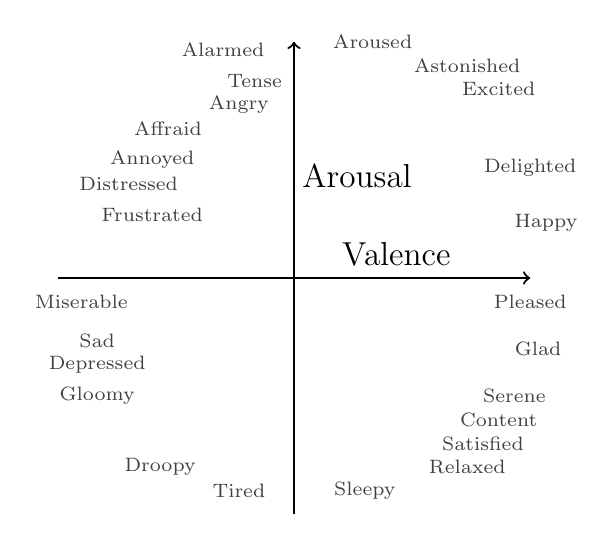
\begin{tikzpicture}
\large
\draw[thick,->] (3,0) -- (3,6) node[anchor=north east] {};
\draw[thick,->] (0,3) -- (6,3) node[anchor=north west] {};
\node at (3.8,4.3) {Arousal};
\node at (4.3,3.3) {Valence};

\scriptsize
\node[darkgray] at (4,6) {Aroused};
\node[darkgray] at (5.2,5.7) {Astonished};
\node[darkgray] at (5.6, 5.4) {Excited};
\node[darkgray] at (6, 4.4) {Delighted};
\node[darkgray] at (6.2, 3.7) {Happy};
\node[darkgray] at (6, 2.7) {Pleased};
\node[darkgray] at (6.1, 2.1) {Glad};
\node[darkgray] at (5.8, 1.5) {Serene};
\node[darkgray] at (5.6, 1.2) {Content};
\node[darkgray] at (5.4, 0.9) {Satisfied};
\node[darkgray] at (5.2, 0.6) {Relaxed};
\node[darkgray] at (3.9, 0.3) {Sleepy};
\node[darkgray] at (2.3, 0.3) {Tired};
\node[darkgray] at (1.3, 0.6) {Droopy};
\node[darkgray] at (0.5, 1.5) {Gloomy};
\node[darkgray] at (0.5, 1.9) {Depressed};
\node[darkgray] at (0.5, 2.2) {Sad};
\node[darkgray] at (0.3, 2.7) {Miserable};
\node[darkgray] at (1.2, 3.8) {Frustrated};
\node[darkgray] at (0.9, 4.2) {Distressed};
\node[darkgray] at (1.2, 4.5) {Annoyed};
\node[darkgray] at (1.4, 4.9) {Affraid};
\node[darkgray] at (2.3, 5.2) {Angry};
\node[darkgray] at (2.5, 5.5) {Tense};
\node[darkgray] at (2.1, 5.9) {Alarmed};
\end{tikzpicture}
\caption[Circumplex Model of Affect]{Circumplex Model of Affect \cite[S. 4]{8a02f9c512933d46fbea928d23ac65e38b61b88caba9b38319a5d4952b5a6667} bzw. \cite[S. 7]{russell1980circumplex}}
\end{figure}
\end{center}

Weiterhin sind Emotionen zu lesen, die an der entsprechenden Stelle im Valence-Arousal Koordinatensystem eingetragen sind \cite[S. 4]{8a02f9c512933d46fbea928d23ac65e38b61b88caba9b38319a5d4952b5a6667} \cite[S. 7]{russell1980circumplex}. Wie man sieht werden die abgebildeten Emotionen nach rechts hin glücklicher, sowie nach oben hin aufgeregter oder aktiver. Zu entscheiden ist nun, ob die Einteilung in Klassen oder die Approximation über ein Modell für eine Visualisierung besser geeignet ist.\\
Für die Umsetzung des Prototypen wurde das Circumplex Model of Affect benutzt, da ein Modell ein differenzierteres Ergebnis liefert, als die Klassifizierung. Auch könnten Fehler bei der Klassifizierung eher zu auffallend unpassenden Visualisierungen führen. Der Hauptgrund liegt aber darin, dass sich die Musik und damit auch die durch sie erzeugte Stimmung über die Zeit ändert \cite{8a02f9c512933d46fbea928d23ac65e38b61b88caba9b38319a5d4952b5a6667}. Diese Veränderungen lassen sich nur schwer über Klassen darstellen, da keine Möglichkeiten zwischen den Klassen existieren. Diese Veränderungen sind leicht über ein Modell zu realisieren, da zwischen zwei Punkten im Valence-Arousal-Raum beliebig viele Zwischenpunkte zu finden sind. Aus diesen Gründen werden zu den kontinuierlichen Daten ein Valence, sowie ein Arousal Wert hinzugefügt. Die praktische Berechnung dieser Werte wird im Abschnitt Implementierung behandelt.

\subsection{Zeit in der Musik}
Musik verändert sich über die Zeit. Aus diesem Grund ist es nicht zielführend einem Attribut der Musik einen einzelnen Wert pro Musikstück zu geben, sondern es ist vielmehr sinnvoll die Attribute und deren Entwicklung über die Zeit des Stückes zu betrachten. Würde man beispielsweise versuchen einen einzelnen Arousal-Wert zu errechnen, so würden ruhigere oder lautere Stellen nicht unterschiedlich visualisiert werden. Auch klingen gleiche Akkorde unterschiedlichen, wenn man sie in anderen Kontexten benutzt und sind somit Kontextabhängig. Die Emotionen verändern sich nicht sprunghaft, sondern entwickeln sich während des Hörens. Auch spielen Gedächtnis und Erwartung des Hörers eine entscheidende Rolle bei der Wahrnehmung von Musik \cite[S. 2]{8a02f9c512933d46fbea928d23ac65e38b61b88caba9b38319a5d4952b5a6667}. Aus diesen Gründen sind Durchschnittswerte von den gewonnenen Daten für eine Visualisierung uninteressant.\\
Um die Informationen in der Musik speichern zu können, wird eine passende Darstellung benötigt. Diese muss zu unterschiedlichen Zeitpunkten unterschiedliche Werte für das gleiche Attribut annehmen können. Bei der Umsetzung des Prototypen wurde diese zeitliche Darstellung für Events und kontinuierliche Daten unterschiedlich vorgenommen. Events besitzen, wie oben angesprochen ein Zeitattribut in Sekunden. Dadurch lassen sich Events auch nach Zeit sortieren, was für die Verarbeitung dieser hilfreich ist. Im Gegensatz dazu besitzen die kontinuierlichen Daten keine explizite Zeitangabe. Für die Umsetzung des Prototypen wurde die Musik in sogenannte Frames eingeteilt. Ein Frame ist eine Zeitspanne von 2048 Samples, was bei einer Samplerate von 44100 Hz einer Zeit von ca. 46.4 Millisekunden entspricht. Diese Frames überlappen sich zur Hälfte, was dazu führt, dass alle 1024 Samples (= 23.3 Millisekunden) ein Frame beginnt. Die Werte der kontinuierlichen Daten werden für jeden Frame neu berechnet und gespeichert, um für weitere Berechnungen zur Verfügung zu stehen oder für die Visualisierung benutzt zu werden.\\
Für die Einteilung in Frames bietet Essentia den ``FrameCutter'' Algorithmus \cite{EssentiaFrameCutter}. Von diesem lässt sich die Größe (FrameSize) als auch die Sprungweite (HopSize) konfigurieren. Alle weiteren kontinuierlichen Berechnungen bauen auf den so gewonnenen Frames auf.

\subsection{Visualisierung}
Will man eine 3D-Visualisierung umsetzen, so bietet es sich an Objekte zu benutzen, die passend zur Musik Eigenschaften
und damit ihr Aussehen verändern. Position, Farbe und Form sind solche Eigenschaften. Über die Position selbst lassen sich wenig Informationen zum Betrachter transportieren, weshalb hier eher die Veränderung der Position, also die Bewegung, eine entscheidende Rolle spielt. Im Folgenden werden die einzelnen Attribute und ihre Verbindung zur Musik behandelt. Dadurch werden Möglichkeiten entwickelt, wie eine Visualisierung der vorher gewonnenen Daten umgesetzt werden kann.

\subsubsection{Farbe}
Der Zusammenhang von Musik und Farben ist wenig erforscht. Besser erforscht ist hingegen der Zusammenhang zwischen Farben und Emotionen, so werden Farben bewusst eingesetzt, um in Bildern, Filmen, Computerspielen und anderen Multimediaanwendungen gesteuerte Emotionen hervorzurufen \cite{10.3389/fpsyg.2017.00440}. Will man menschliche Emotionen untersuchen, so werden häufig kurze Filme oder Bilder verwendet, um die gewünschten Emotionen zu erzeugen. Zu beachten ist hierbei, dass gleiche Farben in unterschiedlichen Ländern und Kulturen unterschiedliche Bedeutungen haben und dadurch unterschiedliche Emotionen hervorrufen können. So ist in China die Farbe des Todes Weiß, während es in westlichen Ländern Schwarz ist.\\
In Tabelle 3 sind Farben und ihre nach Naz Kaya and Helen H. Epps
 \cite{c0f471f7e6a618d880cf25175c9f99ac97ef8ba7d016c7f8c523f8d902892d9e} zugeordneten Emotionen und Assoziationen zu sehen.

\definecolor{yellow_color}{RGB}{248, 230, 77}
\definecolor{green_color}{RGB}{0, 142, 78}
\definecolor{blue_color}{RGB}{5, 158, 212}
\definecolor{red_color}{RGB}{218, 65, 74}
\definecolor{white_color}{RGB}{255, 255, 255}
\definecolor{gray_color}{RGB}{80, 80, 80}
\definecolor{black_color}{RGB}{0, 0, 0}

\begin{center}
\begin{table}[h!]
\begin{tabular}{l | l | l | l}
\textbf{Farbe} & & \textbf{Emotionen} & \textbf{Assoziationen}\\
\hline
Gelb & \cellcolor{yellow_color} & Fröhlichkeit, Aufregung & Sonne, Sommer \\
Grün & \cellcolor{green_color} & Fröhlichkeit, Entspannung, Frieden, Hoffnung & Natur, Pflanzen \\
Blau & \cellcolor{blue_color} & Ruhe, Entspannung & Ozean, Himmel \\
Rot & \cellcolor{red_color} & Liebe, Wärme, Aktivität, Gefahr & Herzen, Blut \\
Weiß & \cellcolor{white_color} & Unschuld, Friede, Einsamkeit, Langeweile & Brautkleid, Schnee \\
Grau & \cellcolor{gray_color} & Traurigkeit, Langeweile & Schlechtes Wetter \\
Schwarz & \cellcolor{black_color} & Depression, Angst & Trauer, Wohlstand \\

\end{tabular}
\captionsetup{justification=centering}
\caption[Farben Emotionen Assoziationen]{Farben, ihre Emotionen und Assoziationen\\nach Naz Kaya and Helen H. Epps
 \cite{c0f471f7e6a618d880cf25175c9f99ac97ef8ba7d016c7f8c523f8d902892d9e}}

\end{table}
\end{center}
Trägt man die Farben entsprechend den Beschreibungen in ein Valence Arousal Koordinatensystem ein, so ergibt sich der in Abbildung 5 zu sehende Verlauf.

\begin{wrapfigure}{l}{0.5\linewidth}
\begin{tikzpicture}[]
  \pgftext{\includegraphics[scale=0.5]{res/images/color_map}} at (0pt,0pt);
  \draw[white,thick,->] (-3,-3) -- (-3,3) node[anchor=north west] at(-3, 1) {Arousal};
  \draw[white,thick,->] (-3,-3) -- (3,-3) node[anchor=north east] at(1, -3) {Valence};
\end{tikzpicture}
\captionsetup{justification=centering}
\caption[Farbverlauf im Valence Arousal Koordinatensystem]{Farbverlauf\\im Valence Arousal\\Koordinatensystem}
\end{wrapfigure}
\noindent
Jedem Punkt im Arousal Valence Koordinatensystem ist eine entsprechende Farbe zugeordnet. Bei niedrigen Arousal Werten, also bei ruhiger Musik, gehen die Farben ins Blaue beziehungsweise ins Graue für kleine Valence Werte oder ins Grüne für hohe Valence Werte. Gelbe Farben werden bei aktiven fröhlichen (hohe Valence und hohe Arousal Werte) erzeugt und rote Farben, wenn die Musik weniger fröhlich, aber immer noch aktiv ist. Wird die Musik noch trauriger wird Schwarz erzeugt. In der Mitte befindet sich ein Orange-Braun. Dies ist nur eine mögliche Anordnung von Farben und es würde sich eventuell anbieten, weitere kompatible Farbeverläufe zu kreieren, um Farbkombinationen zu ermöglichen. Die Umsetzung der Stimmung$ \rightarrow $Farbe-Zuordnung wird im Kapitel Implementierung behandelt.

\subsubsection{Bewegung}
Bewegung und Musik sind eng miteinander verbunden. Rolf Inge God{\o}y und Alexander Refsum Jensenius meinen: ``Performers produce sound through movements, and listeners very often move to music, as can be seen in dance and innumerable everyday listening situations.'' \cite[S. 1]{905eee055abaf2a4f198ce11f35362a8963f61d552297a02dfc8fbc0c4f78679}. Aus diesem Grund ist die Auswahl von Bewegungen für eine Visualisierung wichtig. Im Folgenden werden erst Grundprinzipien natürlicher Bewegungen besprochen. Danach Parameter von Bewegungen und warum diese für die Visualisierung wichtig sind. Zum Schluss werden beispielhaft bestimmte Typen von Bewegungen und Formationen besprochen.
\paragraph{Grundprinzipien}
In der Umwelt sind physische Dinge massebehaftet. Daraus folgt, dass es weder schlagartige Positions- noch Geschwindigkeitsänderungen gibt. Will man eine Gruppe von Objekten oder Partikeln natürlich bewegen, so muss dieser Fakt mit einbezogen werden. Angenommen wird hierbei meistens eine Punktmasse, wobei die gesamte Masse des Objektes im Zentrum des Objektes liegt. Dadurch werden die Bewegungen des Objektes besser berechenbar.\\
Um plötzliche Positions- und Geschwindigkeitsunterschiede zu vermeiden sollten bewegte Objekte eine persistente Position und eine persistente Geschwindigkeit haben, die jeden Frame verändert werden kann. Auf die Position wird die Geschwindigkeit addiert. Eine Wirkung auf das sich bewegende Objekt erzeugt man durch Beschleunigungen, welche die aktuelle Geschwindigkeit anpassen. Diese Beschleunigungen können plötzlich auftreten und werden jeden Frame neu berechnet. Sie sind also nicht über mehrere Frames persistent wie die Position oder die Geschwindigkeit.\\
Eine bekannte Methode, um Objekte natürlich zu beschleunigen ist das sogenannte ``Steering Behaviour'' \cite{580abc6c6615ef9f9c16f9069351938a0dda3c5120b7e8d1450d6b1abf0a71df}. Dabei wird eine Beschleunigung für ein bewegtes System errechnet. Das Ziel ist es das Objekt zu einem gewissen Punkt zu bringen oder es davon zu entfernen. Es gibt mehrere Variationen des Steering Behaviours, es soll hier aber nur um die einfache Form ``Seek'' (Anstreben) gehen.\\
Hat ein bewegtes System die Geschwindigkeit $current\_velocity$, eine maximale Geschwindigkeit von $max\_velocity$ und die Position $current\_position$ und existiert weiterhin ein angestrebter Punkt $target\_position$, so kann man eine einwirkende Beschleunigung $steering\_force$ berechnen, die das Objekt zur $target\_position$ bringt.
\begin{align}
desired\_velocity &= current\_position - target\_position \\
steering\_force &= desired\_velocity - current\_velocity
\end{align}
Neben dem Seek Algorithmus gibt es Abwandlungen, wie ``Flee'', ``Arrive'' oder ``Wander''.\\
Um die Geschwindigkeit zu begrenzen kann Formel (1) wie folgt abgewandelt werden:
\begin{align}
desired\_velocity &= (current\_position - target\_position) * max\_velocity
\end{align}
\noindent
Die Formel (2) bleibt bestehen.\\
Eine andere Möglichkeit die Geschwindigkeit zu begrenzen, ist es eine Reibung (einen Drag) einzuführen. Dazu wird die Geschwindigkeit mit folgender Beschleunigung addiert:
\begin{align}
drag\_force = current\_velocity * -drag
\end{align}

\noindent
Die Variable $drag$ sollte dabei eine Zahl $0 < drag < 1$ sein. Ein kleiner $drag$ bedeutet eine geringe Dämpfung, während ein großer $drag$ eine stärkere Dämpfung der Geschwindigkeit erzeugt.

\paragraph{Bewegungen spannend gestalten}
Eine Bewegung von Objekten sollte möglichst nicht einseitig werden, weshalb ein zufälliger Anteil der Abläufe vorteilhaft sein kann. Eine andere Möglichkeit, um die entstehenden Bilder abwechslungsreich zu gestalten, ist Parameter der Bewegungen zu definieren, die abhängig von den analysierten Daten verändert werden können. Nicht alle Parameter müssen von allen Bewegungen implementiert werden.\\
Die Geschwindigkeit der bewegten Objekte kann als Parameter verwendet werden. Aktive, hektische Musik kann auf diese Weise behandelt werden, indem die Geschwindigkeit der Objekte erhöht wird. Unter Umständen bietet es sich bei Gruppenbewegungen an, einen Parameter einzuführen, der beschreibt, wie kompakt die Objekte beieinander gehalten werden und einen Parameter, der beschreibt, wie häufig sich Richtungsänderungen der Bewegungen ereignen.\\
Im Folgenden sollen Beispiele für Bewegungen beleuchtet und darauf untersucht werden, ob sie sich für eine Visualisierung eignen. Dazu wird geprüft, ob die Bewegung interessant genug ist und ob sie sich performant genug umsetzen lässt.\\

\paragraph{Flow Fields} Flow Fields sind eine Art der Bewegung, die in der Computergraphik vor allem für die Simulation von Flüssigkeiten und Gasen eingesetzt werden \cite{stam1999stable}. Sie werden mit Hilfe eines in Würfel eingeteilten Raumes umgesetzt. Für jeden Würfel wird ein zufälliger Vektor bestimmt, der den Vektoren der umliegenden Würfel ähnelt. Nun werden Partikel in diesem Raum erzeugt. Der Mittelpunkt von jedem Partikel befindet sich in genau einem der Würfel. Jeder Partikel wird in Richtung des Vektors beschleunigt, in dessen zugehörigen Würfel er sich befindet. Durch die Ähnlichkeit der Vektoren von anliegenden Würfeln entsteht eine Fließbewegung der Partikel.\\
Eine Erweiterung ist, die Vektoren der Würfel über Zeit verändern zu lassen, um die Bahnen der Partikel zu verändern. Auch kann die Beschleunigung der Partikel verändert werden, sowie die Kompaktheit des Feldes.\\
Die Umsetzung eines Flow Fields ist aufwendig, da es nicht einfach ist, den Anforderungen entsprechende Richtungsvektoren zu generieren, die sich über Zeit verändern und dabei ihre Ähnlichkeit bewahren. Um diese Vektoren zu generieren, wird ``Perlin Noise'' oder der Nachfolger ``Simplex Noise'' verwendet \cite{bcc7190da8e90284b4e790817b8eed4ee3ea6cffbe5a23ef07a000ca5628ffbc}. Perlin Noise ist eine Zufallsfunktion mit besonderen Eigenschaften. Sie wurde 1982 von Ken Perlin für den Film ``Tron'' entwickelt. Perlin erhielt dafür 1997 einen Oscar. Sie wurde damals zur Generierung von Texturen eingesetzt.\\
Perlin Noise ist eine kontinuierliche Funktion, die im  eindimensionalen Fall eine Zahl $x \in \mathbb{R}$ auf eine andere zufällige Zahl $noise(x) \in \mathbb{R}$ abbildet \cite{25a05da283ffd9d4bdda94c308ccf3a8759f22373b368f895cbef2e9186ab646}. Weiterhin sorgt eine kleine Änderung von $x$ auch nur für eine kleine Änderung von $noise(x)$. Ein möglicher Plot der Perlin Noise Funktion ist in Abbildung 6 zu sehen.
\begin{SCfigure}[][h]
\hspace{110pt}
\includegraphics[scale=0.5]{res/images/perlin_noise}
\caption[Perlin Noise Plot aus \cite{nature_of_code}]{\\Perlin Noise Plot aus \cite[Kap.\\Introduction]{nature_of_code}}
\end{SCfigure}

\noindent
Neben der eindimensionalen Perlin Noise Funktion existieren auch mehrdimensionale. Diese bilden die Zahlen $x_1, x_2, ..., x_n \in \mathbb{R}$ auf eine Zahl $noise(x_1, x_2, ..., x_n) \in \mathbb{R}$ ab. Dabei gilt wie bei der eindimensionalen Version, dass eine kleine Änderung von einem der Eingangswerte auch nur eine kleine Auswirkung auf die Ausgabe der $noise$ Funktion haben wird.\\
Flow Fields lassen sich unter Zuhilfenahme der mehrdimensionalen Perlin Noise Funktion umsetzen. Es gibt unterschiedliche Möglichkeiten das Ergebnis der Perlin Noise Funktion auf einen Vektor abzubilden. Im zweidimensionalen Raum wird häufig der aus der Perlin Noise Funktion gewonnene Wert als Winkel eines Vektors interpretiert. Nachteil hierbei ist, dass die generierten Vektoren eine konstante Länge haben, da sich die Vektoren nur über den Winkel unterscheiden. Weiterhin ist die Interpretation einer oder zweier Zahlen als Winkel im dreidimensionalen Raum schwieriger.\\
Eine andere Möglichkeit einen Vektor $v_{x,y,z}$ zu generieren, wobei $x, y, z$ die Koordinaten des zu $v_{x, y, z}$ gehörigen Würfels sind, funktioniert wie in Formel (5) gezeigt.
\begin{align}
v_{x,y,z} = \left(
\begin{array}{c}
noise(x, y, z) \\
noise(x+a, y+a, z+a) \\
noise(x+2a, y+2a, z+2a)
\end{array}
\right)
\end{align}
\noindent
Bei dieser Möglichkeit wird jede Koordinate von $v$ über einen eigenständigen Aufruf der Perlin Noise Funktion erzeugt, wodurch auch die Länge des Vektors zufällig ist.\\
Das konstante Offset $a$ wurde eingeführt, damit sich die einzelnen Koordinaten des Vektors unterscheiden. Es sollte möglichst groß gewählt sein, da so Wiederholungen räumlich weiter voneinander getrennt sind und so nicht sichtbar werden.\\
Da $noise(x, y, z)$ und $noise(x+\delta, y+\delta, z+\delta)$ umso ähnlicher werden je kleiner $\delta$ wird, kann man die Ähnlichkeit der Vektoren bestimmen, indem die Positionen $x, y, z$ mit einem Faktor $f$ multipliziert werden.
\begin{align}
v_{x,y,z} = \left(
\begin{array}{c}
noise(f \cdot x, f \cdot y, f \cdot z) \\
noise(f \cdot x+a, f \cdot y+a, f \cdot z+a) \\
noise(f \cdot x+2a, f \cdot y+2a, f \cdot z+2a)
\end{array}
\right)
\end{align}
\noindent
Für kleine $f$ sind die erzeugten Vektoren $v_{x, y, z}$ und $v_{x+\delta, y+\delta, z+\delta}$ ähnlicher als für große $f$. Kritisch könnte der Rechenaufwand der Perlin Noise Funktion werden, da sie für jeden Würfel drei mal ausgeführt werden muss. Eine Alternative wäre es, einen Vektor $v_{x, y, z}$ aus einer einzelnen Zahl zu entwickeln. Dafür wäre ein Abbildung $f: \mathbb{R} \mapsto \mathbb{R}^3$ nötig. Eine andere Möglichkeit wäre es, das Flow Field nur in zwei Dimensionen zu erstellen und die Höhe der Objekte über eine andere Logik zu bestimmen. Dies würde auch die Laufzeit der $noise(x_1, ..., x_n)$ Funktion verbessern, die eine Komplexität von $2^n$ hat, wobei $n$ die Anzahl der Dimensionen ist.\\
Weiterhin muss das Problem gelöst werden, dass Objekte aus dem Flow Field heraus gedrückt werden können. Diesem Problem könnte man begegnen, indem auf jeden Vektor $v$ ein Vektor, der in Richtung der Mitte des Feldes zeigt, addiert.

\paragraph{Random Acceleration}
Objekte in eine zufällige Richtung zu beschleunigen, kann vor allem dafür verwendet werden, rhythmische Elemente zu visualisieren. Wird eine Gruppe von dicht zusammenstehenden Objekten gleichzeitig in unterschiedliche Richtungen beschleunigt, wird eine pulsierende Bewegung erzeugt. Erweitert werden kann dies, indem alle betroffenen Objekte zu einem gemeinsamen Punkt hin beschleunigt werden oder von diesem weg. Dadurch lässt sich auch die Kompaktheit der Gruppen verändern.

\paragraph{Formationen}
Um eine Alternative zu den Flow Fields zu haben, bieten sich viele unterschiedliche Formationen an, in denen die Partikel bewegt werden. Eine einfach zu implementierende Variante ist es, die Partikel in Kreisen parallel zum Horizont fliegen zu lassen. Dazu wird der Mittelpunkt $m \in \mathbb{R}^3$ des Kreises bei der Erstellung definiert, sowie sein Radius $r \in \mathbb{R}$.
Will man ein Partikel mit der Position $p \in \mathbb{R}^3$ kreisen lassen, so kann wie folgt vorgegangen werden.\\
Man projiziert den Vektor $p - m$, also den Vektor der von $m$ auf $p$ zeigt, auf die Ebene, die parallel zum Horizont verläuft und durch m geht, indem man die y-Koordinate von $p - m$ auf die y-Koordinate von $m$ setzt. Diesen Vektor nennen wir $p_0$. Man bildet jetzt das Kreuzprodukt zwischen $p_0$ und dem Up-Vektor $(0, 1, 0)$. Daraus entsteht ein parallel zum Horizont verlaufender Vektor $t$.
\begin{center}
\begin{figure}[h!]
\centering
\vspace{20pt}
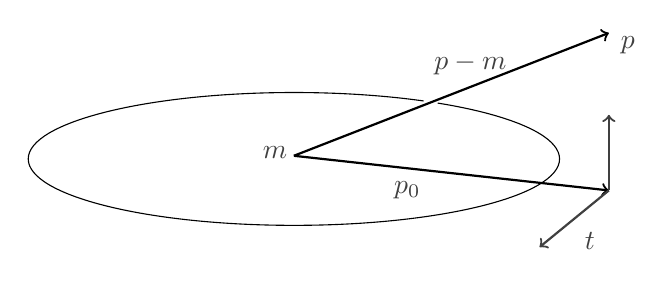
\begin{tikzpicture}[scale=0.8]
\draw (0,0) ellipse (120pt and 30pt);
\filldraw[white] (2.17, 0.9) circle (3pt);
\draw[thick,->] (0,0.05) -- (5,2);
\node[darkgray] at (2.8,1.5) {$p-m$};
\node[darkgray] at (-0.3,0.1) {$m$};
\node[darkgray] at (5.3,1.8) {$p$};
\draw[thick,->] (0,0.05) -- (5,-0.5);
\node[darkgray] at (1.8,-0.5) {$p_0$};
\draw[darkgray,thick,->] (5,-0.5) -- (5,0.7);
\draw[darkgray,thick,->] (5,-0.5) -- (3.9,-1.4);
\node[darkgray] at (4.7,-1.3) {$t$};
\end{tikzpicture}
\caption[Kreisbewegung]{Kreisbewegung}
\end{figure}
\end{center}
\noindent
Nimmt man jetzt $p_0+t$ und setzt die Länge des resultierenden Vektors auf $r$, so erhält man einen Punkt, der vom Partikel angesteuert werden kann (Steering Behaviour), um den Partikel in eine Kreisbahn zu bringen. Über die Länge von $t$ lässt sich die Geschwindigkeit der Partikel bestimmen.

\newpage

\section{Implementierung}
In diesem Abschnitt wird die Implementierung des Prototypes mit Hilfe der oben beschriebenen Konzepte erläutert. Dazu wird zuerst die grobe Aufteilung des Projektes aufgezeigt, um danach auf die einzelnen Bestandteile des Prototypen einzugehen. Dabei werden auch die Schnittstellen der Bestandteile gezeigt und wie diese miteinander interagieren. Neben dem Skizzieren des Gesamtsystems sollen auch Algorithmen, die eine gewisse Komplexität übersteigen, erläutert werden, um die Funktionsweise des Prototypen zu veranschaulichen.

\subsection{Übersicht}
Der Prototyp gliedert sich in drei größere Bestandteile, nämlich den Visualizer, die Audioanalyse und den AudioVisualizer, der die beiden anderen Teile zusammen verwendet. Der Visualizer wurde als eigenständige Bibliothek umgesetzt, die vom AudioVisualizer benutzt wird und von der Audioanalyse unabhängig ist. Er verwaltet die animierten Objekte, deren Aussehen und Bewegungen, sowie den Rendervorgang mit Hilfe von OpenGL. Auch verarbeitet er die Benutzereingaben und die damit verbundene Kameraposition.\\
Für die Audioanalyse wird, wie bereits in der Analyse erläutert, Essentia verwendet. Die grundlegenden Funktionen von Essentia wurden erweitert, um spezielle Informationen, die für die Umsetzung nötig waren, extrahieren zu können.\\
Um die beiden unabhängigen Komponenten Visualizer und Audioanalyse zu verbinden, wurde der AudioVisualizer entwickelt. Dieser entscheidet, welche Daten und Events erzeugt werden und setzt diese Informationen in eine Visualisierung um, die dann im Visualizer realisiert wird, indem Objekte erzeugt, gelöscht und verändert werden. Im Unterschied zu Essentia und dem Visualizer, ist der AudioVisualizer eine ausführbare Datei und keine Bibliothek. Bei der Ausführung wird der AudioVisualizer gestartet, der dann die Audioanalyse durchführt. Erst wenn diese fertig ist, wird mit Hilfe des Visualizers die Visualisierung gestartet. Theoretisch hätte die Analyse auch während der laufenden Visualisierung durchgeführt werden können, um das Programm schneller starten zu können. Ich habe mich dagegen entschieden, da einige Algorithmen für die Analyse besser funktionieren, wenn Informationen aus der Zukunft mit verarbeitet werden können. Die modulare Aufteilung wurde gewählt, um das Projekt überschaubar zu gestalten und die einzelnen Komponenten unabhängig voneinander testen und weiterentwickeln zu können.

% Warum modular
\newpage
\subsection{Visualizer}
In diesem Kapitel soll die Funktionsweise und die Benutzung der Visualizer Bibliothek beschrieben werden. Dafür wird erst das System im Großen aufgezeigt, sowie die Möglichkeit auf dieses einzuwirken, um danach die einzelnen Funktionalitäten genauer zu erklären.

\subsubsection{Aufbau}
Der Visualizer ist die Implementierung des grafischen Anteils des Projektes. Er verwaltet die Objekte, aus denen die Animation besteht und bietet eine Schnittstelle, die es erlaubt, auf das Verhalten dieser Objekte einzuwirken.\\
Um die Funktionalität der Visualisierung zu definieren, wurde eine ``Visualizer'' Klasse geschrieben. Diese Klasse ruft bei ihrer Instanziierung die Initialisierungsfunktionen für OpenGL auf, erzeugt ein Fenster mit einer gegebenen Breite und Höhe und kompiliert die ``Shader''. Um den Stand der Visualisierung zu verändern existiert eine ``tick()'' Funktion, die jeden Frame aufgerufen werden sollte. Um den Ablauf der Visualisierung auf unterschiedlichen Systemen stabil zu halten, wird eine delta-Time berechnet, um die Geschwindigkeit der Objekte so zu skalieren, dass die Visualisierung auch auf langsamen Systemen mit gleicher Geschwindigkeit abläuft. Weiterhin speichert die Visualizer Klasse die Objekte mit der die Animation umgesetzt wird.\\
Die Animation der Musik wird über viele kleine Objekte, die sogenannten Entities, umgesetzt. Das Verhalten von Entities wird über ``Movements'' realisiert. Movements können einer Entity oder einer Gruppe von Entities zugeordnet werden, um das Verhalten dieser Entities zu verändern, wobei vor allem die Bewegungen und die Farbe der Entities modifiziert werden.\\
Weiterhin wird die Form der Entities über sogenannte ``Shapes'' definiert. Das Shape einer Entity wird über deren ``Vertices'' umgesetzt, die später noch genauer behandelt werden. Jede Entity hat genau einen Shape.\\
Um neue Entities erzeugen zu können, wurde die ``Creation'' Klasse geschrieben, die alle nötigen Informationen enthält, die für die Erstellung einer Gruppe von Entities nötig sind. Mit ihr ist es möglich mit nur einem Funktionsaufruf viele unterschiedliche Entities zu erzeugen, die sich jeweils in Position, Shape, Größe und Farbe unterscheiden.\\
Um auch nach der Erstellung auf Entities einwirken zu können, kann man im Visualizer nach Entities mit definierten Eigenschaften suchen. Dazu existiert die ``Query''-Klasse.

%\newpage
\subsubsection{Speicherung der Objekte}
Die Objekte oder Partikel, mit denen die Visualisierung erzeugt wird, werden durch eine ``Entity'' Klasse beschrieben. Diese Entity Klasse enthält alle Informationen, die für das Rendern des Objektes benötigt werden. Diese Attribute sind eine Beschreibung des Shapes, also die Form der Oberfläche, eine Position, eine Größe, sowie eine Farbe.\\
Diese Entity Klasse enthält keine Informationen über die Geschwindigkeit oder die Bewegungen des Objektes. Um diese Informationen abzubilden, existiert eine ``Movable'' Klasse, die eine Entity Instanz enthält. Die Movable Klasse enthält zusätzlich eine Geschwindigkeit, eine Liste von Bewegungen, die von diesem Movable ausgeführt werden sollen, sowie eine Liste von ``Tags'', die benutzt werden kann, um Movables zu identifizieren. Weiterhin existiert eine ``Geschwindigkeit für die Farbe''  des Objektes, da auch die Farbe keine schlagartigen Änderungen erfahren soll. Im Folgenden sollen unterschiedliche Möglichkeiten untersucht werden, eine Menge dieser Movable Instanzen zu speichern.
\paragraph{EntityBuffer}
Da die Movable Klasse keine Form der Vererbung benutzt, müssen keine Movable-Pointer verwendet werden. Deshalb wäre eine triviale Art der Speicherung eine Liste oder ein Array (in c++ einen std::vector<Movable>) zu verwenden, um die einzelnen Partikel zu speichern. Nennen wir diese Liste ``EntityBuffer''.\\
Folgender Anwendungsfall wird hierbei problematisch. Wenn man nur eine Teilmenge aller Movables betrachten möchte, um beispielsweise diesen eine Bewegung zu geben, so muss über den gesamten EntityBuffer iteriert werden und nur die in der Gruppe enthaltenen Movables behandelt werden. Da diese Operation mehrmals pro Frame passieren kann, ist diese Variante nicht sehr effektiv.
\paragraph{Externe Gruppen}
Um dieses Problem zu lösen, könnte man über den EntityBuffer iterieren und sich mehrere std::vector<Movable*> erstellen, die jeweils eine Teilmenge repräsentieren. Diese Gruppen werden dann gespeichert, um im nächsten Frame wiederverwendet werden zu können. Dies ist sehr riskant, da die Movable-Pointer invalide werden, wenn der EntityBuffer neuen Speicher alloziert oder Elemente aus dem EntityBuffer entfernt werden.
\paragraph{Heap Allocation}
Dies würde nicht passieren, wenn schon der EntityBuffer Movable-Pointer speichern würde, anstatt Movables direkt zu speichern. Dies hätte den Nachteil, dass die Objekte mit ``new'' und ``delete'' erstellt und gelöscht werden müssten oder die Verwendung von Smartpointern notwendig wird, wobei das Löschen der Objekte aus allen Vektoren ein Problem darstellt.
\paragraph{Map}
Wenn die Gruppen der Movables direkt in Gruppen gespeichert werden, so ist das ansprechen einer Gruppe direkt möglich, ohne über alle Movables iterieren zu müssen. Dazu werden die Movables in einer Map gespeichert, die einen Identifikator, zum Beispiel einen String, auf einen Vektor von Movables abbildet. Nachteil ist, dass das iterieren über alle Movables umständlicher ist, da erst über die Map und dann über die Vektoren iteriert werden muss. Weiterhin können externe Pointer auf Movables invalide werden, sobald die Map oder einer der Vektoren neuen Speicher alloziert oder verschiebt.

\begin{center}
\begin{table}[h!]
%\resizebox{\textwidth}{!}{%
\begin{tabular}{l | l | l}
\textbf{Bezeichnung} & \textbf{Vorteile} & \textbf{Nachteile}\\
\hline
EntityBuffer & - kein new/delete & - langsamer Zugriff auf Teilmengen \\
& - einfaches iterieren über\\
& \hspace{4pt} alle Entities\\
 \hline
Externe Gruppen & - schneller Zugriff auf & - Gruppen müssen neu erstellt werden, \\
& \hspace{4pt} Teilmengen &\hspace{4pt}  wenn EntityBuffer Speicher verschiebt. \\
& & - Dies ist schwierig festzustellen. \\
\hline
Heap Allocation & - Schneller Zugriff auf & - Löschen einer Entity schwierig, \\
& \hspace{4pt} Teilmengen & \hspace{4pt} da diese in mehreren Listen steht. \\
& - Movable$^\ast$ bleiben valide & - Weiterer Layer of Indirection\\
\hline
Map & - Schneller Zugriff auf & - Iterieren über alle Movables umständlich \\
& \hspace{4pt} Teilmengen & - Weiterer Layer of Indirection\\
& - kein new/delete& - Movable kann nicht in mehreren \\
& & \hspace{4pt} Gruppen sein \\
\end{tabular}
%}
\captionsetup{justification=centering}
\caption[Möglichkeiten des Memory Managements]{Möglichkeiten des Memory Managements}
\end{table}
\end{center}
\normalsize
Für die Umsetzung des Prototypen wurde die Map gewählt, da deren Nachteile am wenigsten ins Gewicht fallen. Das Iterieren über alle Movables kann man mit einem eigenen Iterator vereinfachen und der Zugriff auf Teilmengen erfolgt schnell. Weiterhin müssen die Movables nicht einzeln referenziert werden (std::vector\textless Movable$^\ast$\textgreater), sondern der gesamte Vektor kann benutzt werden (std::vector\textless Movable\textgreater$^\ast$). Der Fakt, dass ein Movable auf diese Weise nicht in mehreren Gruppen sein kann, wird in Kauf genommen.

\subsubsection{OpenGL}
Für die Erzeugung der Grafiken wurde OpenGL verwendet. In diesem Abschnitt soll beschrieben werden, wie OpenGL's ``core-profile'' benutzt wird, um dann in den folgenden Abschnitten erklären zu können, wie OpenGL in das System integriert wurde. Dabei wird bewusst nur aufgezeigt, wie OpenGL benutzt wird, ohne dabei in die Tiefe zu gehen, da eine ausführliche Erklärung der Funktionsweise von OpenGL nicht das Ziel dieser Arbeit ist. Meine Informationen habe ich vor allem aus diesem Tutorial \cite{LearnOpenGL}.\\
Um Grafiken mit OpenGL erzeugen zu können, muss zuerst ein Fenster mit Hilfe von GLFW erzeugt werden. Dies wird über die Funktion \mbox{\textit{glfwCreateWindow()}} realisiert.

\begin{lstlisting} [caption={Erzeugen eines Fensters mit GLFW}\label{lst:test123},captionpos=t,language=c++]
GLFWwindow* window = glfwCreateWindow(width, height,
                                      "Visualizer",
                                      NULL, NULL);
glfwMakeContextCurrent(window);
\end{lstlisting}
\noindent
Die Funktion \mbox{\textit{glfwCreateWindow()}} kann dabei einen Null-Pointer zurückgeben, falls das Fenster nicht erstellt werden konnte. Die ersten beiden Parameter sind die Breite und Höhe des Fensters. Das dritte Argument ist der Titel.\\
In OpenGL werden Objekte grundlegend aus Dreiecken aufgebaut, die über die Position ihrer Ecken definiert werden. Zwar sind auch Linien  und Punkte möglich, diese können aber nicht für Flächen verwendet werden. Die lokalen Positionen der Ecken werden über Vertices festgelegt. Später werden diese lokalen Positionen im ``Vertex-Shader'' zu Positionen in einer 3D Szene umgerechnet.\\
Vertices werden als Array von float Werten umgesetzt und über ``Vertex Buffer Objects'' auf der Grafikkarte verwaltet. Um ein Vertices Array an die Grafikkarte zu senden sind drei Schritte nötig. Zuerst muss ein Buffer generiert werden. Dies erfolgt über den Aufruf von \mbox{\textit{glGenBuffers()}}. Danach muss der generierte Buffer gebunden werden, um ihn daraufhin mit Daten zu füllen. Der Ablauf sieht aus wie folgt.


\begin{lstlisting} [caption={Generierung eines Buffers und Laden der Vertices}\label{lst:test123},captionpos=t,language=c++]
unsigned int vbo;
glGenBuffers(1, &vbo);
glBindBuffer(GL_ARRAY_BUFFER, vbo);
glBufferData(GL_ARRAY_BUFFER, sizeof(vertices),
             vertices, GL_STATIC_DRAW);
\end{lstlisting}
\noindent
Die Variable \textit{vbo} ist die ID für den generierten Buffer. Diese wird beim Aufruf von \mbox{\textit{glGenBuffers()}} gesetzt und wird ab hier dazu verwendet den Buffer anzusprechen. Dieser wird durch \mbox{\textit{glBindBuffer()}} gebunden, was dazu führt das weitere Funktionsaufrufe, wie beispielsweise \mbox{\textit{glBufferData()}} sich auf diesen Buffer beziehen. Die Funktion \mbox{\textit{glBufferData()}} wird dann benutzt, um die Daten, die sich im float Array \mbox{\textit{vertices}} befinden, in den durch \mbox{\textit{vbo}} identifizierten Buffer zu schreiben. Die Konstante \mbox{\textit{GL\_STATIC\_DRAW}} gibt an, dass die \mbox{\textit{vertices}} nicht für häufiges Überschreiben optimiert werden müssen. Als Alternativen existieren \mbox{\textit{GL\_DYNAMIC\_DRAW}}, sowie \mbox{\textit{GL\_STREAM\_DRAW}}, die für \mbox{\textit{vertices}} konzipiert sind, die sich häufig ändern. Bevor ein vbo erstellt werden kann, muss noch ein \mbox{\textit{Vertex Array Object}} (VAO) auf ähnliche Weise erzeugt werden.\\
Um diese Daten eine globale Position in der Welt zu geben und die 3D Szene auf einem 2D Bildschirm darzustellen, wird der ``Vertex-Shader'' benutzt. In Listing 2 ist der im Prototypen benutzte Vertex-Shader zu sehen.

\begin{lstlisting} [caption={Vertex Shader}\label{lst:test123},captionpos=t,language=c++]
layout (location = 0) in vec3 aPos;

uniform mat4 model;
uniform mat4 view;
uniform mat4 projection;

void main()
{
	gl_Position = projection * view * model * vec4(aPos, 1.0);
}

\end{lstlisting}
\noindent
Um einen Shader benutzen zu können, muss dieser mit der Funktion \mbox{\textit{glCompileShader()}} kompiliert werden. Dies passiert zur Laufzeit des eigentlichen Programms und schlägt fehl, falls Fehler im Shadercode sind.\\
Die Matrizen \mbox{\textit{model}}, \mbox{\textit{view}} und \mbox{\textit{projection}} werden verwendet, um die lokalen Koordinaten der \mbox{\textit{vertices}} in Koordinaten umzuwandeln, die zum Rendern auf einem 2D Bildschirm verwendet werden können. Die \mbox{\textit{model}} Matrix insbesondere verschiebt, rotiert und skaliert die Koordinate \mbox{\textit{aPos}} in ein globales Koordinatensystem, mit dessen Hilfe Positionen der Entities dargestellt werden. Die Variable \mbox{\textit{aPos}} nimmt dabei die Werte der Vertices an.\\
Damit die \mbox{\textit{vertices}} richtig interpretiert werden, muss über sogenannte Attribute-Pointer definiert werden, welche Teile der \mbox{\textit{vertices}} welche Variablen des Vertex-Shaders definieren.

\begin{lstlisting} [caption={Attribute Pointer}\label{lst:test123},captionpos=t,language=c++]
glVertexAttribPointer(0, 3,
                      GL_FLOAT, GL_FALSE,
                      3 * sizeof(float), (void*)0);
glEnableVertexAttribArray(0);
\end{lstlisting}
\noindent
Mit dem hier zu sehenden Funktionsaufruf \mbox{\textit{glVertexAttribPointer()}} wird ein solcher Attribut-Pointer gesetzt. Er definiert, welcher Attribut-Pointer gesetzt werden soll, dessen Größe, einen Stride, sowie ein Offset. Der Stride definiert, wie weit der nächste Satz von \mbox{\textit{vertices}} entfernt ist. Mit \mbox{\textit{glEnableVertexAttribArray()}} wird der Attribut-Pointer aktiviert.\\
Neben dem Vertex-Shader muss auch ein Fragment-Shader bereitgestellt werden, der vor allem die Textur und Farbe eines Objektes bestimmt. Zusammen mit dem Vertex Shader kann ein Shader-Programm mit \mbox{\textit{glLinkProgram()}} gelinkt werden.\\
Um nun Objekte zu rendern muss das Shader-Programm mit \mbox{\textit{glUseProgram()}} aktiviert werden, ein \mbox{\textit{VAO}} gebunden und die in den Shadern definierten \mbox{\textit{uniforms}} festgelegt sein. Dann kann mit der Funktion \mbox{\textit{glDrawArrays()}} gerendert werden.

\subsubsection{Initialisierung und Callbacks}
Bei der Erstellung einer \mbox{\textit{Visualizer}} Instanz wird das Fenster erstellt, sowie das Shader-Programm geladen, kompiliert und gelinkt. Da die Initialisierung des Fensters, sowie die Kompilierung der Shader fehlschlagen kann, werden diese Aufgaben nicht im Konstruktor des Visualizers abgearbeitet, sondern in einer \mbox{\textit{Visualizer::create()}} Funktion, die ein \mbox{\textit{std::optional<Visualizer>}} zurückgibt. Dieser Aufbau wurde gewählt, da der Konstruktor in der Fehlerbehandlung eingeschränkt ist, da er immer eine \mbox{\textit{Visualizer}} Instanz zurückgeben werden muss. Schlägt die Kompilierung eines Shaders fehl oder kann kein Fenster erzeugt werden, so wird ein leeres \mbox{\textit{optional}} zurückgegeben.\\
Bei der Initialisierung musste ein weiteres Problem gelöst werden, dass kurz beschrieben werden soll. OpenGL informiert das eigene Programm über Mausbewegungen und Größenänderungen des Fensters. Dies geschieht über Callback-Funktionen, die vom Programmierer gesetzt werden können. Ein Callback für die Größenänderung des Fensters setzt man mit der Funktion \mbox{\textit{glfwSetFramebufferSizeCallback(window, callback\_function)}}, wobei \mbox{\textit{callback\_function()}} die vom Programmierer definierte Funktion ist, die bei einer Größenänderung ausgeführt wird. Ungünstiger weise ist es nicht möglich eine Member-Funktion zu registrieren, wodurch verhindert wird, dass der \mbox{\textit{Visualizer}} eine eigene Funktion registriert. Man könnte eine statische Funktion registrieren und in dieser einen globalen State verändern, der dann vom \mbox{\textit{Visualizer}} benutzt wird, um die Visualisierung anzupassen. Da aber globale Variablen ``Bad Practice'' sind und verhindern würden, mehrere Visualizer Instanzen zu benutzen, habe ich mich entschieden, einen \mbox{\textit{ResizeManager}}, sowie einen \mbox{\textit{MouseManager}} zu schreiben, bei dem sich der \mbox{\textit{Visualizer}} registrieren kann, um die OpenGL-Callbacks auf eigenen Member-Funktionen umleiten zu lassen.\\
Dazu gibt der \mbox{\textit{Visualizer}} dem \mbox{\textit{ResizeManager}}, sowie dem \mbox{\textit{MouseManager}} eine Referenz von sich selbst, die von den Managern benutzt wird, um die Member-Funktion des \mbox{\textit{Visualizers}} aufzurufen. Im Destruktor des \mbox{\textit{Visualizers}} wird die Referenz wieder entfernt.

\subsubsection{Shapes}
Die Form einer Entity wird im Visualizer über sogenannte ``Shapes'' identifiziert. Dabei definiert ein Shape die \mbox{\textit{vertices}} eines Objektes, beispielsweise die in Listing 5 zu sehenden \mbox{\textit{vertices}} eines einfachen Dreiecks \cite[Kap. ``Hello Tiangle'']{LearnOpenGL}.

\begin{lstlisting} [caption={Vertices eines Dreiecks},captionpos=t,language=c++]
float vertices[] = {
    -0.5f, -0.5f, 0.0f, // unten links
     0.5f, -0.5f, 0.0f, // unten rechts
     0.0f,  0.5f, 0.0f  // oben mitte
};
\end{lstlisting}
\noindent
Möchte man einen Würfel definieren, so kann man diesen aus 12 Dreiecken zusammensetzen, von denen jeweils zwei eine Seite des Würfels bilden. Dies lässt sich noch per Hand umsetzen.\\
Schwieriger sind die  \mbox{\textit{vertices}} einer Kugel zu berechnen, da man, um eine Kugel zu erzeugen, relativ viele  \mbox{\textit{vertices}} benötigt, da ansonsten Ecken der Kugeln zu sehen sind. Es existieren unterschiedliche Arten der Generierung von Kugel-\mbox{\textit{vertices}}. Im Prototypen wurde die Problematik wie folgt gelöst. Zuerst werden, wie in Abbildung 8 zu sehen, zwei aufeinander stehende Pyramiden erstellt, die aus jeweils vier Dreiecken bestehen.\\
Nun wird jedes Dreieck der Pyramiden in vier weitere Dreiecke geteilt, indem die Mittelpunkte der Seiten verbunden werden (ebenfalls in Abbildung 8 zu sehen). Die so entstandenen Dreiecke können wieder auf die gleiche Weise unterteilt werden. Diesen Vorgang wiederholt man nun, bis eine ausreichende Feinheit erreicht wurde. Anschließend werden die Vektoren, die vom Mittelpunkt der Kugel zu den Eckpunkten der Vierecke verlaufen, normalisiert. Das Resultat ist eine Approximation einer Kugel.\\

\begin{center}
\begin{figure}[h!]
\centering
\vspace{20pt}
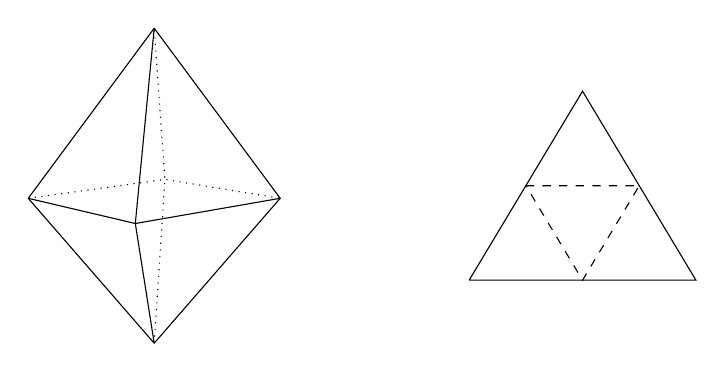
\begin{tikzpicture}[scale=0.8]
\draw(0,0) -- (2,2.3) -- (0, 5);
\draw(0,0) -- (-2,2.3) -- (0, 5);
\draw(-2,2.3) -- (-0.3, 1.9) -- (2, 2.3);
\draw(0, 0) -- (-0.3, 1.9) -- (0, 5);
\draw[dotted](-2,2.3) -- (0.17, 2.6) -- (2, 2.3);
\draw[dotted](0,0) -- (0.17, 2.6) -- (0, 5);

\draw(5,1) -- (6.8, 4) -- (8.6, 1) -- (5,1);
\draw[dashed](5.9, 2.5) -- (7.7, 2.5) -- (6.8, 1) -- (5.9, 2.5);
\end{tikzpicture}
\caption[Ausgangsstatus der Kugelberechnung und Dreiecksteilung]{Ausgangsstatus der Kugelberechnung und Dreiecksteilung}
\end{figure}
\end{center}
\noindent
Will man mit OpenGL unterschiedliche Objekte rendern, die aber die gleiche Form annehmen, so ist es deutlich effizienter, die \textit{vertices} nicht für jedes Objekt neu auf die Grafikkarte zu laden, sondern diese wiederzuverwenden.\\
Um dies umzusetzen, wurde der \textit{ShapeHeap} entwickelt, der die schon erstellten Shapes und damit die hoch geladenen \textit{vertices} verwaltet. Dieser bildet mit Hilfe einer Map sogenannte \textit{ShapeSpecifications} auf konkrete Shapes ab. Eine \textit{ShapeSpecification} definiert exakt, wie ein Shape aussehen soll. Die Spezifikation einer Kugel enthält beispielsweise, wie oft die Dreiecke in Folge geteilt werden sollen, um zu definieren, wie genau die Kugel gezeichnet werden soll.\\
Will man eine Kugel mit einer gegebenen \textit{ShapeSpecification} erzeugen, so ruft man die Funktion \mbox{\textit{get\_shape()}} des \mbox{\textit{ShapeHeaps}} auf, die eine \textit{ShapeSpecification} als Argument akzeptiert. Diese überprüft, ob ein \textit{Shape} mit der gegebenen \textit{ShapeSpecification} schon erstellt wurde und falls ja gibt es dieses zurück. Andernfalls wird das \textit{Shape} neu erstellt und zurück gegeben. Auf diese Weise wird sichergestellt, dass gleiche \textit{vertices} nicht mehrmals auf die Grafikkarte hoch geladen werden.

\newpage
%\subsubsection*{Kamera}
\subsubsection{Movements}
Um die Bewegung von Entities lenken zu können, wurden Movements entwickelt, die sich in zwei Arten unterscheiden. Es gibt Einzelbewegungen oder \textit{Movements}, die immer einzelnen Entities zugeordnet werden und Gruppenbewegungen oder \mbox{\textit{GroupMovements}}, die nur auf Gruppen von Entities angewendet werden können.

\paragraph{Einzelbewegungen}
Um die Einzelbewegungen umzusetzen, wurde eine abstrakte Klasse \textit{IMovement} geschrieben, von der die unterschiedlichen Bewegungen erben sollen. Diese deklariert die Funkionen \textit{void init(Movable* movable)}, \textit{void apply\_force(Movable* movable) = 0} und \textit{bool should\_be\_removed()}. Die \textit{init()} Funktion wird beim Hinzufügen des \textit{Movements} zur \textit{Movable} Instanz ausgeführt, wobei sich die \textit{Movable} Instanz selbst als Argument übergibt. Dabei kann das \textit{Movement} initiale Einstellungen vornehmen, wie Daten des \textit{Movables} abspeichern oder es verändern.\\
In der \textit{apply\_force()} Funktion findet die tatsächliche Tätigkeit des \textit{Movements} statt, wie eine Veränderung der Geschwindigkeit oder der Farbe, weshalb jede Unterklasse von \textit{IMovement} diese Funktion überschreiben muss. Dabei hat das \textit{Movement} kompletten Zugriff auf das \textit{Movable} Objekt.\\
Um zu wissen, wann das \textit{Movement} wieder gelöscht werden soll, gibt es die Funktion \textit{should\_be\_removed()}, die jeden Frame vom \textit{Movable} aufgerufen wird. Wenn \textit{true} zurück gegeben wird, wird das \textit{Movement} aus der Liste der \textit{Movements} entfernt.\\
Neben den eben genannten Funktionen gibt es eine \textit{clone()} Funktion, die eine neu allozierte Kopie des Movements erzeugt. Um die \textit{clone()} Funktion nicht für jedes \textit{Movement} neu schreiben zu müssen, wurde die Templateklasse \textit{IMovementCloneable\textless Movement\textgreater} geschrieben, die von \textit{IMovement} erbt und die \textit{clone()} Funktion abhängig vom Template Argument erstellt.\\
Da für die Verwendung von Polymorphismus in C++ Pointer notwendig sind, werden die Unterklassen von \textit{IMovement} mit \textit{new} erstellt und müssen dementsprechend mit \textit{delete} gelöscht werden. Um dies zu vereinfachen, gibt es die \textit{Movement} Klasse, die genau dieses Memory-Management übernimmt. Sie bekommt im Konstruktor einen mit \textit{new} erzeugten Pointer einer \textit{IMovement}-Unterklasse, klont diese, falls das \textit{Movement} kopiert wird und gibt den Speicher im Destruktor wieder frei.

\paragraph{Gruppenbewegungen}
Während Einzelbewegungen auf bestimmte Entities angewendet werden können, indem sie einem \textit{Movable} Objekt hinzugefügt werden, beziehen sich \textit{GroupMovements} immer auf ganze Gruppen des \textit{EntityBuffers}. Sie werden verwendet, wenn viele Entities in einer gemeinsamen Bewegung zusammengefasst werden.\\
Die Umsetzung des \textit{GroupMovements} unterscheidet sich an vielen Stellen von der Umsetzung der Einzelbewegungen. Zwar kann man, wie bei den Einzelbewegungen, unterschiedliche Arten von \textit{GroupMovements} über neue Klassen definieren, diese haben aber keine gemeinsame Oberklasse. Stattdessen werden sie in einem \textit{std::variant\textless \textgreater} zusammengefasst, die in C++ 17 eingeführt wurden.\\
Ein \mbox{\textit{std::variant\textless A,B \textgreater}} ist eine  typensichere Union, die entweder den Typen A oder B annimmt, von denen es beliebig viele geben kann (\textit{std::variant\textless A, B, C, ... \textgreater}). Zugriff auf ein \textit{variant} bekommt man über die Funktion \textit{std::visit()}, die als Argumente zuerst einen Funktor oder einen Funktionspointer, der für alle Varianten des Variants überladen ist und als zweites die Instanz des Variants erwartet. Das Variant, welches alle GroupMovements zusammenfasst heißt \textit{\_GroupMovementVar} und ist für den Benutzer des Visualizers nicht sichtbar. Alle Klassen, die im \textit{\_GroupMovementVar} Variant zusammengefasst sind, müssen die Funktion \textit{apply\_force()} definieren, die einen \textit{std::vector\textless Movable\textgreater}\& als Argument erwartet. In dieser Funktion wird die Logik der Bewegung definiert.\\
Um den Aufruf der Gruppenbewegungen zu vereinfachen wurde die Klasse \textit{GroupMovement} entwickelt, die eine Instanz des Variants hält. Sie definiert die Funktion \textit{apply\_to()}, die einen EntityMap Pointer akzeptiert und die im Variant gehaltene Bewegung auf alle \textit{Movables} in der Map anwendet, indem die \textit{apply\_force()} Funktion des Movements im Variant ausgeführt wird. Will man die Bewegung nicht auf alle Gruppen der Map anwenden, so kann man in der \textit{GroupMovement}-Instanz eine Liste von Gruppen definieren, die von der Bewegung betroffen ist.\\
Die Unterschiede der \textit{Movements} sollen kurz aufgezeigt werden. Während man bei den Einzelbewegungen für jede Movable-Instanz eine neue Instanz der Bewegung benötigt, wird für eine Gruppenbewegung nur eine Instanz für alle Movables benötigt. Dafür ist es für Einzelbewegungen möglich, einzelne Entities zu beeinflussen. Der größte Vorteil von \textit{GroupMovements} ist der, dass man sie deutlich einfacher Verwalten kann. Will man Parameter einer Einzelbewegung ändern, so muss man diese erst in der EntityMap suchen. Danach wird es schwierig diese voneinander zu unterscheiden, da die Typeninformation über die Oberklasse verlorengegangen ist.\\
Ein \textit{GroupMovement} behält durch die Verwendung des Variants die Typeninformation und es wird nur eine Instanz benötigt, sodass eine aufwendige Suche in der EntityMap entfällt. Im Folgenden wird auf ausgesuchte Movements eingegangen und versucht deren Funktionsweise zu erläutern.

\paragraph{Flow Fields} % Do
Die grundlegenden Möglichkeiten Flow Fields umzusetzen, wurden schon in der Konzeptphase beschrieben. An dieser Stelle soll vor allem darauf eingegangen werden, wie sich die Implementation und das Konzept unterscheiden und wie die Perlin Noise Funktion umgesetzt wurde.\\
Anders als im Konzept geplant, wurden die Flow Fields nicht umgesetzt, indem der Raum in Würfel eingeteilt wurde und ein Beschleunigungsvektor $v$ für jeden Würfel berechnet wurde. Stattdessen wurde die Position der Entities direkt als Eingabe der Perlin Noise Funktion verwendet. Dies hat folgende Vorteile. Erstens ist der Raum, in dem die Beschleunigung der Entities definiert ist, dadurch nicht mehr begrenzt. Würde man Beschleunigungsvektoren für eine endliche Anzahl von Würfeln berechnen, so würde der durch die Würfel beschriebene Raum immer endlich sein und es wäre schwierig die Bewegungen der Entities außerhalb dieses Raumes zu beschreiben. Zweitens ist die Beschleunigung der Entities dadurch stetig, da nicht die diskreten Positionen der Würfel, sondern die stetigen Positionen der Entities als Eingabe der PerlinNoise Funktion verwendet werden. Wichtig hierbei war, dass die Performanz der Perlin Noise Funktion ausreicht, um Beschleunigungen, für eine ausreichend große Menge von Entities, berechnen zu können.
\subparagraph{Perlin Noise}
Die Standard Bibliothek von C++ bietet keinen Algorithmus, der Perlin Noise berechnet, weshalb erst der Perlin Noise Algorithmus implementiert werden musste. Dabei war es nicht wichtig, dass der originale Algorithmus umgesetzt wurde, sondern vielmehr mussten nur die in der Konzeptphase beschriebenen Anforderungen erfüllt sein. Die \textit{noise()} Funktion musste $n$ Argumente akzeptieren und sicherstellen, dass eine kleine Änderung der Argumente auch nur eine kleine Änderung der \textit{noise()} Funktion bewirkt.\\
Grundlegend wurde vorgegangen, indem eine zufällige Folge $\left(f_i\right)_{i \in \mathbb{N}}$ definiert wird, die auf die Zahlen $[-1, 1]$ abbildet.
Anschließend wird zwischen den Werten der Folge mit dem Polynom $6x^5-15x^4+10x^3$ interpoliert. Abbildung 9 zeigt eine Veranschaulichung der Zufallsfolge mit Interpolation, sowie einen Plot des Polynoms. Die blauen Punkte befinden sich an den Punkten $\left(i, \left(f_i\right)\right)$ einer möglichen Zufallsfolge, zwischen denen mit der schwarzen dünnen Linie interpoliert wird. Auf der rechten Seite befindet sich der Plot des Interpolationspolynoms $I(x) = 6x^5-15x^4+10x^3$.

\begin{center}
\begin{figure}[h!]
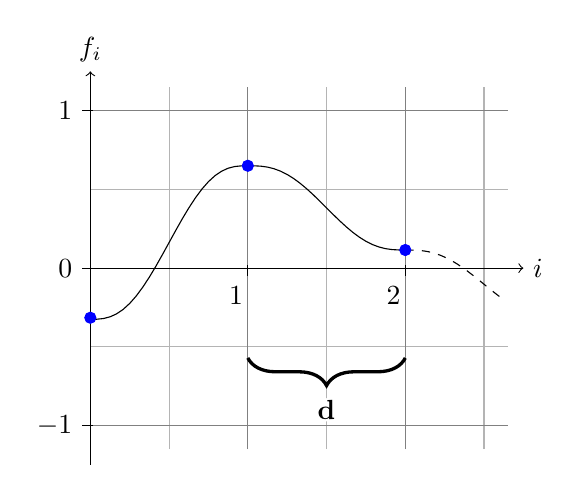
\begin{tikzpicture}[scale=1]
\draw[thin, code_comment, step=1] (0, -2.3) grid (5.3,2.3);
\draw[thin, gray, step=2] (0, -2.3) grid (5.3,2.3);
\draw[->] (0, -2.5) -- (0, 2.5) node[above] {$f_i$};
\draw[->] (0, 0) -- (5.5, 0) node[right] {$i$};

\draw [domain=0:2, thin] plot (\x, {-0.65+1.95*(6*\x^5*0.03125-15*\x^4*0.0625+10*\x^3*0.125)});
\draw [domain=0:2, thin] plot (\x+2, {1.3-1.07*(6*\x^5*0.03125-15*\x^4*0.0625+10*\x^3*0.125)});
\draw [domain=0:1.2, thin, dashed] plot (\x+4, {0.23-0.87*(6*\x^5*0.03125-15*\x^4*0.0625+10*\x^3*0.125)});

\filldraw [blue](0, -0.63) circle (2pt);
\filldraw [blue](2, 1.3) circle (2pt);
\filldraw [blue](4, 0.23) circle (2pt);

\foreach \x in {1,2}
  \draw (\x*2,1pt) -- (\x*2,-3pt)
    node[anchor=north,xshift=-0.15cm] {$\x$};
\foreach \y/\ytext in {-1, 0, 1}
  \draw (1pt,\y*2) -- (-3pt,\y*2) node[anchor=east] {$\ytext$};

\filldraw [white](3, -1.8) circle (4pt);

\draw [very thick, decorate,decoration={brace,amplitude=10pt,mirror,raise=4pt},yshift=0pt] (2,-1) -- (4,-1);
\node at (3, -1.8) {\textbf{d}};

\end{tikzpicture}
\hspace{50pt}
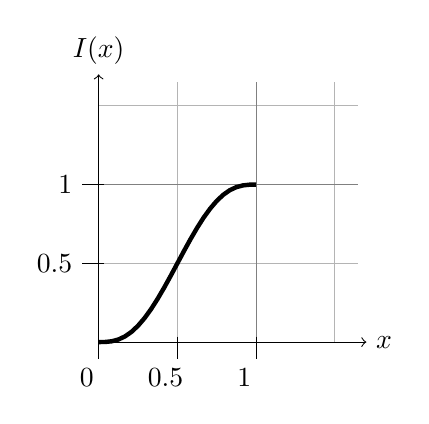
\begin{tikzpicture}[scale=2]
\draw[thin, code_comment, step=0.5] (0, 0) grid (1.65,1.65);
\draw[thin, gray, step=1] (0, 0) grid (1.65,1.65);
\draw[thin, ->] (0, 0) -- (0, 1.7) node[above] {$I(x)$};
\draw[thin, ->] (0, 0) -- (1.7, 0) node[right] {$x$};

\draw [domain=0:1, ultra thick] plot (\x, {6*\x^5-15*\x^4+10*\x^3});

\foreach \x in {0, 0.5, 1}
  \draw (\x,1pt) -- (\x,-3pt)
    node[anchor=north,xshift=-0.15cm] {$\x$};
\foreach \y/\ytext in {0.5, 1}
  \draw (1pt,\y) -- (-3pt,\y) node[anchor=east] {$\ytext$};
\end{tikzpicture}
\caption[Zufallsfolge $\left(f_i\right)$ und Interpolation]{Zufallsfolge $\left(f_i\right)$ mit Interpolation und Interpolationspolynom $I(x)$}
\end{figure}
\end{center}
\noindent
Man könnte die in Abbildung 9 links gezeigten, interpolierten Werte als eine stetige Funktion $noise\_part_d\colon \mathbb{R} \rightarrow [-1, 1]$ auffassen, wobei $d$ den Abstand zwischen den Zufallswerten von $(f_i)$ angibt. Die Funktion $noise\_part_{0.5}(x)$ würde also an den Stellen $0, 0.5, 1, 1.5, ...$ einen durch $(f_i)$ definierten Wert annehmen und dazwischen interpolieren. Um Perlin Noise zu erzeugen, werden mehrere $noise\_part_d$ Funktionen mit unterschiedlichen Argumenten für $d$ verwendet und $m$ mal, gewichtet zusammen summiert, wobei $m \in \mathbb{N}\setminus\{0\}$ beliebig gewählt werden kann. Man nennt $m$ auch die Anzahl der ``Octaves'' \cite[Kap. Introduction]{nature_of_code}.

\begin{align}
noise(x) = \sum^{m}_{j=1} k \cdot noise\_part_{k}(x) \mid k = \frac{1}{j^2}
\end{align}
\noindent
Dies kann umgesetzt werden, indem das Argument von $noise\_part_k$ mit $j$ multipliziert wird, da so eine Änderung von $x$ mit $j$ skaliert wird, was dazu führt, dass man nur noch die $noise\_part_1$ Funktion benötigt.
\begin{align}
noise(x) = \sum^{m}_{j=1}  \frac{1}{j^2} \cdot noise\_part_1(j^2 \cdot x)
\end{align}
\noindent
Diese Funktion erfüllt die Eigenschaften, dass eine kleine Änderung von $x$ ebenfalls auch $noise(x)$ nur geringfügig ändert. Allerdings ist es noch nicht möglich mehrere $x$ anzugeben. Um dies zu erreichen, muss ebenfalls die Zufallsfolge $(f_i)$ $n$ viele Argumente auf einen Zufallswert abbilden, $f_{i_1, i_2, ..., i_n} \rightarrow \mathbb{R}$. Ist dies umgesetzt, so muss in der neuen Funktion $noise\_part(x_1, x_2, ..., x_n)$ über $n$ Dimensionen interpoliert werden. Dies soll kurz anhand eines zweidimensionalen Beispiels veranschaulicht werden.\\
Gegeben seien die Eingabewerte der $noise(x_1, x_2)$ Funktion mit $x_1=3.3$ und $x_2 = 1.7$ (Der blaue Punkt in Abbildung 10). Gehen wir von $m = 1$ aus, was bedeutet, dass nur eine Octave berechnet wird. Da unsere Eingabewerte $x_1 = 3.3$ und $x_2 = 1.7$ sind, müssen wir in diesem Fall auf der $x_1$-Achse zwischen den Werten 3 und 4 und auf der $x_2$ Achse zwischen den Werten 1 und 2 interpolieren. Dazu benötigen wir zuerst die Werte von $(f_{i_1, i_2})$, zwischen denen interpoliert werden soll. Diese sind über $(f_{i_1, i_2})$ an den Stellen $(3, 1), (3, 2), (4, 1), (4, 2)$ (rote Punkte der Abbildung) definiert, also an allen Kombinationen von $(3,4)$ und $(1,2)$.\\

\begin{center}
\begin{figure}[h!]
\centering
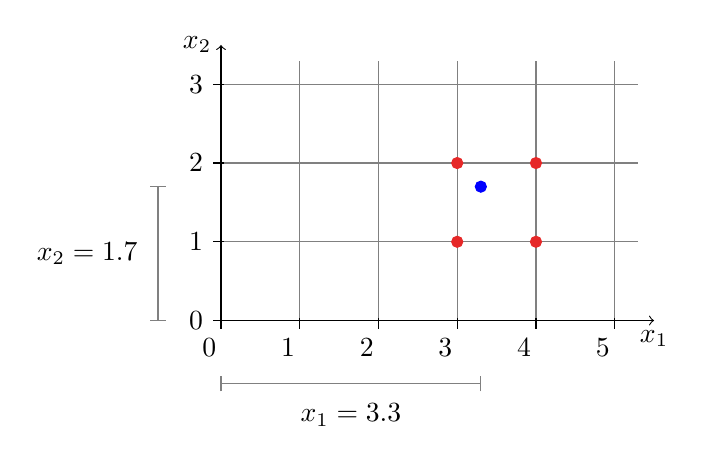
\begin{tikzpicture}
\draw[thin, gray, step=1] (0, 0) grid (5.3,3.3);
\draw[->] (0, 0) -- (0, 3.5) node[anchor=east] {$x_2$};
\draw[->] (0, 0) -- (5.5, 0) node[anchor=north] {$x_1$};

\filldraw[blue] (3.3, 1.7) circle (2pt);

\filldraw[dark_red] (3, 1) circle (2pt);
\filldraw[dark_red] (3, 2) circle (2pt);
\filldraw[dark_red] (4, 1) circle (2pt);
\filldraw[dark_red] (4, 2) circle (2pt);

\draw[thin, gray] (0, -0.8) -- (3.3, -0.8);
\draw[thin, gray] (0, -0.9) -- (0, -0.7);
\draw[thin, gray] (3.3, -0.9) -- (3.3, -0.7);
\node at(1.65, -1.2) {$x_1 = 3.3$};

\draw[thin, gray] (-0.8, 0) -- (-0.8, 1.7);
\draw[thin, gray] (-0.9, 0) -- (-0.7, 0);
\draw[thin, gray] (-0.9, 1.7) -- (-0.7, 1.7);
\node at(-1.7, 0.85) {$x_2 = 1.7$};

\foreach \x in {0, 1, 2, 3, 4, 5}
  \draw (\x,1pt) -- (\x,-3pt)
    node[anchor=north,xshift=-0.15cm] {$\x$};
\foreach \y/\ytext in {0, 1, 2, 3}
  \draw (1pt,\y) -- (-3pt,\y) node[anchor=east] {$\ytext$};
\end{tikzpicture}
\caption[Beispiel 2D Interpolation]{Beispiel 2D Interpolation}
\end{figure}
\end{center}
\noindent
Um das Beispiel weiter rechnen zu können, sei die Folge $(f_{i_1, i_2})$ für die gefragten Stellen, wie folgt definiert:
\begin{center}
$f_{3, 1} = -0.2$ \hspace{10pt} $f_{3, 2} = 0.4$ \hspace{10pt} $f_{4, 1} = 0.7$ \hspace{10pt} $f_{4, 2} = -0.5$\\
\end{center}
\noindent
Interpoliert man erst über $x_1$, so muss zwischen den Wertepaaren $f_{3, 1} = -0.2$ und $f_{4, 1} = 0.7$, sowie $f_{3, 2} = 0.4$ und $f_{4, 2} = -0.5$ interpoliert werden, wobei der Eingangswert $x_1$ mit einbezogen werden muss. Um zwischen den Werten $f_{3, 1} = -0.2$ und $f_{4, 1} = 0.7$ zu interpolieren, muss das Interpolationspolynom $I(x) = 6x^5-15x^4+10x^3$ an die umliegenden Werte angepasst werden. Dazu wird es um $-0.2$ nach unten verschoben und um $0.7 - (-0.2) = 0.9$ gestreckt, woraus $I^\prime(x) = 0.9 \cdot I(x) - 0.2$ resultiert.
\begin{center}
\begin{figure}[h!]
\centering
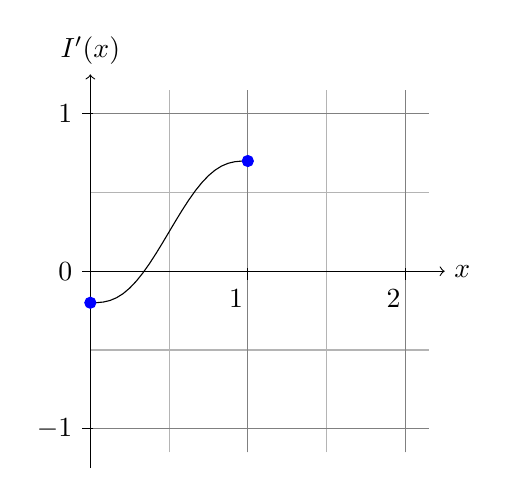
\begin{tikzpicture}[scale=1]
\draw[thin, code_comment, step=1] (0, -2.3) grid (4.3,2.3);
\draw[thin, gray, step=2] (0, -2.3) grid (4.3,2.3);
\draw[->] (0, -2.5) -- (0, 2.5) node[above] {$I^\prime(x)$};
\draw[->] (0, 0) -- (4.5, 0) node[right] {$x$};

\draw [domain=0:2, thin] plot (\x, {-0.4+1.8*(6*\x^5*0.03125-15*\x^4*0.0625+10*\x^3*0.125)});

\filldraw [blue](0, -0.4) circle (2pt);
\filldraw [blue](2, 1.4) circle (2pt);

\foreach \x in {1,2}
  \draw (\x*2,1pt) -- (\x*2,-3pt)
    node[anchor=north,xshift=-0.15cm] {$\x$};
\foreach \y/\ytext in {-1, 0, 1}
  \draw (1pt,\y*2) -- (-3pt,\y*2) node[anchor=east] {$\ytext$};

\end{tikzpicture}
\caption[Interpolation]{Interpolation}
\end{figure}
\end{center}
Setzt man nun $x_1 - floor(x_1) = 3.3 - 3.0 = 0.3$ in $I^\prime(x)$ ein, so erhält man den ersten Interpolationswert $-0.0532$. Die gleiche Prozedur durchläuft man mit $f_{3, 2} = 0.4$ und $f_{4, 2} = -0.5$ und erhält $0.2532$. Nun interpoliert man auf gleiche Weise für $x_2$, mit den errechneten Werten $-0.0532$ und $0.2532$ und erhält $0.2032$, wobei man nun $0.7$ in die Interpolationsfunktion geben muss, da $x_2 - floor(x_2) = 1.7 - floor(1.7) = 0.7$. Somit ist unser Endresultat $0.2032$ für die erste Octave.\\
Für die Implementierung der Zufallsfolge $(f_i)$ wurde eine Abwandlung vom XOR-Shift RNG verwendet, wie sie von George Marsaglia \cite{ac8e278bab88e59aa3a147bef7b113350a723aa4547b89da74bdcadaf0244f1b} vorgestellt wurden. Diese haben den Vorteil, dass sie extrem schnell arbeiten, da sie nur auf dem binären XOR und Shiftoperationen aufbauen. Die Funktion wurde so abgewandelt, sodass Fließkommazahlen zwischen -1 und 1 produziert werden.
\newpage

\begin{lstlisting} [caption={Xorshift RNG},captionpos=t,language=c++]
float random(unsigned int x) {
	x ^= x >> 12;
	x ^= x << 25;
	x ^= x >> 27;
	return (static_cast<float>(x % (_accuracy*2+1)) -
		static_cast<float>(_accuracy)) /
		static_cast<float>(_accuracy);
}
\end{lstlisting}
\noindent
Damit mehrere Eingabewerte verarbeitet werden können, wurden diese zusammengefasst, indem sie aufsummiert wurden. Dabei wurde jeder Eingabewert $x_i$ mit $10^i$ multipliziert, damit beispielsweise die Eingabewerte $(a, b)$ und $(b, a)$ nicht dasselbe Ergebnis produzieren. An dieser Methode sollte man kritisieren, dass die Eingaben $(a, b)$ und $(b\cdot 10, \frac{a}{10})$ die selben Ergebnisse produzieren. Dies fällt in der Visualisierung aber nicht auf und wurde deshalb vernachlässigt.

\vspace{10pt}
\noindent
Mit der beschriebenen n-dimensionalen Perlin Noise Funktion, konnten nun Flow Fields umgesetzt werden, wie sie im Konzept schon beschrieben wurden. Dabei wurde die Perlin Noise Funktion verwendet, indem die Kraft, die auf eine Entity wirkt, ähnlich wie schon in der Konzeptphase, mit folgender Formel berechnet wird:
\begin{align}
force_{x,y,z} = \left(
\begin{array}{c}
noise(y \cdot f + a + time, z \cdot f + a + time) \\
noise(x \cdot f + 2a + time, z \cdot f + 2a + time) \\
noise(x \cdot f + 3a + time, y \cdot f + 3a + time)
\end{array}
\right)
\end{align}
\noindent
Die Variablen $x, y, z$ sind die Position der zu beschleunigenden Entity, wobei zu beachten ist, dass die x-Koordinate nicht in die Beschleunigung auf der x-Achse eingeht, sowie die $y$ und $z$ Position nicht in ihre Beschleunigungen eingehen. Einerseits verbessert es die Performanz, da eine Dimension weniger berechnet wird, andererseits wird so einem Effekt entgegengewirkt, der dafür sorgte, dass sich die Entities auf einer Position häuften.\\
Die Konstante $f$, im Prototypen auf $0.2$ gesetzt, wird, wie schon im Konzept erläutert, benutzt, um zu definieren, wie schnell sich die wirkenden Kräfte von Position zu Position unterscheiden. Ist $f$ sehr klein, unterscheiden sich die Kräfte für auseinander liegende Entities kaum, ist $f$ groß so können große Unterschiede auch bei eng aneinanderliegenden Entities vorkommen. Als weiterer Faktor wurde die Zeit mit einbezogen, sodass sich die Visualisierung über die Zeit verändert. Dadurch, dass sich die Zeit ähnlich wie die Position der Entity auf die berechnete Kraft auswirkt, entstehen Wellenbewegungen, da eine Entity, die sich zum Zeitpunkt $t$ an der Position $(x, y, z)$ befindet die gleiche Kraft erfährt, wie eine Entity an der Position $(x+\delta, y+\delta, z+\delta)$ und dem Zeitpunkt $t-(\delta \cdot f)$.\\
Der Parameter der Geschwindigkeit wurde über eine Skalierung der berechneten Kraft umgesetzt. So führen beispielsweise rhythmische Element dazu, dass die Stärke der Bewegungen kurzzeitig zunimmt.

\paragraph{Plain Force}
Der visuelle Effekt der Flow Fields konnte verbessert werden, indem man eine weitere Kraft hinzufügte, die die Entities in Richtung der xz-Ebene drückte, also die y-Koordinate Richtung 0 beschleunigte. Dies wurde implementiert, indem die y-Koordinate negativ auf die Beschleunigung addiert wurde:
\begin{lstlisting} [caption={Plain Force},captionpos=t,language=c++]
	acceleration += vec3(0.f,
		entity.position.y * -strength,
		0.f));
\end{lstlisting}
\noindent
Der Parameter $strength$ gibt dabei an, wie stark diese Kraft wirkt.\\

\noindent
Weiterhin wurde eine Reibungskraft für die Geschwindigkeit, sowie eine Reibung für die Veränderungen der Farbe implementiert, die unverändert aus dem Konzept übernommen wurden.

\newpage

\subsubsection{Creations}
Um neue Gruppen von Entities in die EntityMap einzufügen, wurde die Klasse \textit{Creation} eingeführt. Diese erlaubt es eine bestimmbare Anzahl von Entities mit einstellbaren Eigenschaften zu erzeugen. Dabei erlaubt sie es vor allem die Eigenschaften der erzeugten Entities auch zufällig zu bestimmen.\\
Zwei Eigenschaften der Creation müssen zu Beginn definiert werden, da sie keine sinnvollen Standartwerte besitzen. Diese Eigenschaften sind eine Definition des Shapes, sowie eine String, der den Gruppennamen definiert. Dieser wird später als Key der EntityMap verwendet. Damit diese Eigenschaften nicht ausgelassen werden dürfen, sind sie im Konstruktor einer \textit{Creation} gefordert.\\
Weitere Eigenschaften, die bestimmt werden können sind die Anzahl der zu erzeugenden Entities, deren Position, Größe, Startgeschwindigkeit und Shape. Diese werden über \textit{with\_}-Funktionen gesetzt, beispielsweise \textit{with\_position()}, die eine Referenz auf die Creation zurückgeben, sodass diese aneinander gereiht werden können. Weiterhin können String-\textit{Tags} der erzeugten Entities gesetzt werden, die später zur Identifikation dieser benutzt werden können.\\
Häufig ist es sinnvoll die Entities mit zufälligen Werten zu initialisieren, um diese beispielsweise an unterschiedlichen Positionen zu erzeugen. Dazu wurden Generator-Klassen geschrieben, deren Erwartungswert und Standartabweichung konfigurierbar sind und deren \textit{get()}-Funktion ein neues zufälliges Objekt, beispielsweise einen Vektor oder ein Shape, zurückgibt. Die \textit{with\_}-Funktionen der \textit{Creation}-Klasse nehmen diese Generator-Klassen entgegen und rufen bei der Erzeugung der Entities deren \textit{get()}-Funktion auf. Die tatsächliche Erzeugung der Entities wird in der \textit{create()}-Funktion der \textit{Creation} vollzogen.

\subsubsection{Queries}
Durch die Einführung der EntityMap ist die Notwendigkeit von \textit{Queries} gesunken, da nun direkt auf bestimmte Gruppen zugegriffen werden kann, weshalb sie nur kurz erwähnt werden.\\
Sie dienten dazu nach Entities in einem EntityBuffer suchen zu können, indem bestimmte Attribute der Entities überprüft werden. Zu diesen Attributen zählen das Shape, die Position, sowie die Tags. In der Umsetzung des Prototypen wurden Queries nicht mehr verwendet.

\subsection{AudioVisualizer}
% Was ist der AudioVisualizer?
Der \textit{AudioVisualizer} verbindet die beiden Parts der Audioanalyse und der Visualisierung. Im Gegensatz zu Essentia und dem Visualizer ist es keine Bibliothek, sondern eine ausführbare Datei, die den Pfad der zu visualisierenden Datei als Command Line Argument entgegennimmt.\\
In den folgenden Abschnitten wird zuerst der grobe Ablauf aufgezeigt, sowie die sich daraus ergebenden Anforderungen an das System, um dann zu erläutern, wie das System aufgebaut wurde. Anschließend werden einzelne Algorithmen näher beleuchtet.

\subsubsection{Ablauf}
Beim Start des AudioVisualizers wird zuerst die Audioanalyse durchgeführt, die noch vor Beginn der Visualisierung abgeschlossen wird. Die Audioanalyse lässt sich gut in mehrere aufeinander aufbauende Verarbeitungsschritte einteilen. Abbildung 12 zeigt die einzelnen Verarbeitungsschritte und deren Abhängigkeiten, sowie generierte Events.

\begin{wrapfigure}{r}{0.4\linewidth}
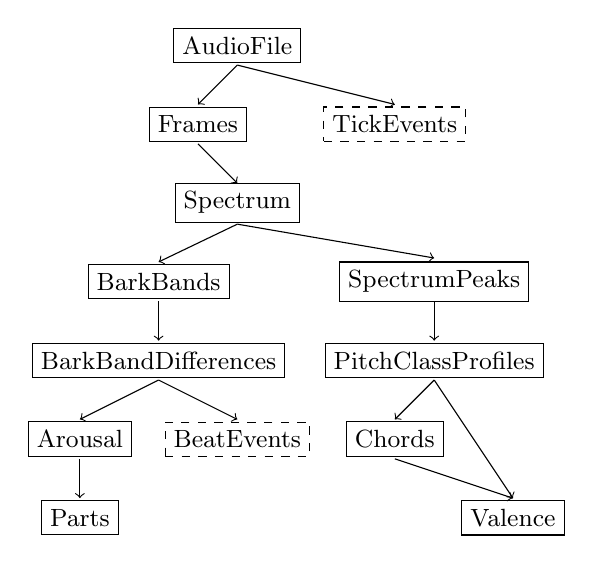
\begin{tikzpicture}[scale=1]
\small
\node (rect) at (0,0) [draw] {AudioFile};
\draw[->] (0, -0.25) -- (2, -0.75);
\node (rect) at (2, -1)[draw, dashed] {TickEvents};
\draw[->] (0, -0.25) -- (-0.5, -0.75);
\node (rect) at (-0.5,-1) [draw] {Frames};
\draw[->] (-0.5, -1.25) -- (0, -1.75);
\node (rect) at (0,-2) [draw] {Spectrum};
\draw[->] (0, -2.27) -- (-1, -2.75);
\node (rect) at (-1,-3) [draw] {BarkBands};
\draw[->] (-1, -3.25) -- (-1, -3.75);
\node (rect) at (-1,-4) [draw] {BarkBandDifferences};
\draw[->] (-1, -4.25) -- (-2, -4.75);
\node (rect) at (-2,-5) [draw] {Arousal};
\draw[->] (-2, -5.25) -- (-2, -5.75);
\node (rect) at (-2,-6) [draw] {Parts};
\draw[->] (-1, -4.25) -- (0, -4.75);
\node (rect) at (0,-5) [draw, dashed] {BeatEvents};
\draw[->] (0, -2.27) -- (2.5, -2.7);
\node (rect) at (2.5,-3) [draw] {SpectrumPeaks};
\draw[->] (2.5, -3.25) -- (2.5, -3.75);
\node (rect) at (2.5,-4) [draw] {PitchClassProfiles};
\draw[->] (2.5, -4.25) -- (2, -4.75);
\node (rect) at (2,-5) [draw] {Chords};
\draw[->] (2, -5.25) -- (3.5, -5.75);
\draw[->] (2.5, -4.25) -- (3.5, -5.75);
\node (rect) at (3.5,-6) [draw] {Valence};
\end{tikzpicture}
\captionsetup{justification=centering}
\caption[Daten und Event Abhängigkeiten]{Daten und Event Abhängigkeiten}
\end{wrapfigure}
\noindent
Die genaue Umsetzung und Begründung der Verarbeitungsschritte wird nicht in diesem Kapitel behandelt, sondern nur eine grobe Übersicht gegeben, um danach die entwickelte Architektur zu begründen.\\
Wie man erkennen kann, wird zuerst die Audiodatei geladen. Direkt daraus gehen die Frames hervor, sowie die Tick-Events. Das Audiomaterial in Frames, also in sich überlappende Abschnitte definierter Länge, zu teilen, wurde schon im Konzept besprochen und ist Voraussetzung für weitere Bearbeitungsschritte. Die Zeiten der Tick-Events werden mit dem dafür vorgesehenen Algorithmus ``RhythmExtractor'' von Essentia berechnet, der die Grundschläge oder Zählzeiten extrahiert. Für die weitere Analyse wird das Spektrum jedes Frames generiert, indem eine diskrete Fourier Transformation durchgeführt wird. Die Einteilung in sogenannte \textit{Bark Bands} hat eine Datenreduktion zur Folge, bei der Frequenzbänder zusammengefasst werden. Dadurch werden die weiteren Berechnungen beschleunigt, wichtige Informationen bleiben aber erhalten, da Bark Bands dem menschlichen Hören nachempfunden sind \cite[S. 80]{lerch2012introduction}. Für die Arousaldaten und die Beat-Events war es, wie schon im Konzept erläutert, sinnvoll, nicht die Lautstärke der einzelnen Frequenzbänder zu betrachten, sondern die Unterschiede benachbarter Frames zu analysieren. Aus diesem Grund werden im nächsten Schritt die Lautstärkedifferenzen der Werte der einzelnen Frequenzbänder ermittelt. Aus diesen gehen die Arousalwerte, sowie die Beat-Events hervor, von denen die Arousalwerte gruppiert werden, um den Song in mehrere Parts zu untergliedern. Mit dem Ziel einen Valence Wert zu bestimmen, werden auch tonale Features, wie Pitch-Class-Profiles und Akkorde (Chords) extrahiert.\\
Ist die Audioanalyse abgeschlossen, wird eine \textit{Visualizer}-Instanz erstellt, deren Objekte über eine \textit{Creation} erstellt und \textit{Movements} initialisiert. Die \textit{Movements} werden dabei passend zu den ermittelten Daten angepasst.

\subsubsection{Aufbau}
Prinzipiell wurde die Arbeit des AudioVisualizers in zwei Teile gebrochen, nämlich die Audioanalyse und die Visualisierung dieser. Für die Audioanalyse wurde eine \textit{InformationBuilder}-Klasse entwickelt, die den Ablauf der Analyse steuert. Für die Organisation der Visualisierung wurde die Klasse \textit{AudioVisualizer} entwickelt.
\paragraph{Audioanalyse}
Der InformationBuilder bekommt den Pfad einer Audiodatei übergeben. Weiterhin wird definiert, welche Daten und Events generiert werden sollen. Ruft man nun die \textit{build()} Funktion auf, so werden die spezifizierten Daten generiert und in einem \textit{InformationContainer} zurück gegeben, der die generierten Daten und Events enthält.\\
Wie eben gezeigt wurde, gibt es bei der Audioanalyse mehrere Teilaufgaben, die nacheinander abgearbeitet werden müssen. Diese Aufgaben haben Abhängigkeiten untereinander und können daher nicht in einer beliebigen Reihenfolge bearbeitet werden. Auch wäre es ungünstig mehrmals benötigte Daten, wie das Spektrum, für jede Anwendung neu zu berechnen.\\
Die Abarbeitung der einzelnen Aufgaben wurde über \textit{DataGenerator} gelöst, die jeweils einen der eben genannten Schritte bearbeiten. Dazu implementieren sie eine \textit{compute()}-Funktion. Ähnlich wie für die Shapes gibt es \textit{DataSpecifications}, die dazu benutzt werden können, einen \textit{DataGenerator} zu erstellen. Dies hat den Vorteil, dass die einfach zu erzeugenden Spezifikationen benutzt werden können, um die schwieriger zu initialisierenden DataGeneratoren zu erstellen. Die Spezifikationen haben simple Konstruktoren, deren Argumente einfach zu definieren sind. Die Generatoren andererseits benötigen Zugriff auf die vorher generierten Daten und einige auch auf eine \textit{AlgorithmFactory} von Essentia. Der InformationBuilder sorgt dafür, dass die Generatoren in der richtigen Reihenfolge aufgerufen werden und das sie den Zugriff auf die benötigten Daten bekommen.\\
Die Reihenfolge wird dabei über Abhängigkeiten gelöst. Jeder DataGenerator kann angeben, welche Daten er benötigt, indem er entsprechende Spezifikationen erstellt. Diese Abhängigkeiten werden dann im InformationBuilder rekursiv abgefragt und sortiert. Sollen nun bestimmte Daten nicht generiert werden, so werden auch deren Abhängigkeiten nicht mehr berechnet, sofern diese nicht anderweitig gebraucht werden.\\
Sind alle notwendigen Daten generiert, so werden diese verwendet, um Events zu generieren. Dies geschieht über \textit{EventGenerators}, die wiederum \textit{EventSpecifications} besitzen. Im Gegensatz zu den kontinuierlichen Daten, haben Events keinen Zugriff auf andere Events. Sie können als Abhängigkeiten ebenfalls DataSpecifications angegeben.

\paragraph{Visualisierung}
Die Visualisierung baut auf den Daten des InformationContainers auf, die in der Audioanalyse berechnet wurden. Hier findet die Umwandlung dieser Daten in Veränderungen der Entities statt, wobei vor allem die Bewegungen und die Farben der Entities verändert werden.\\
Die Visualisierung startet man, indem die \textit{run()}-Funktion der AudioVisualizer Klasse aufgerufen wird. Diese erwartet die analysierten Daten in Form eines InformationContainers, der zuvor mit dem InformationBuilder generiert wurde. In der \textit{run()}-Funktion wird zuerst eine Instanz des \textit{Visualizers} erzeugt und geprüft, ob die Erstellung erfolgreich war. Falls nicht, wird eine Fehlermeldung ausgegeben und das Programm schließt sich. Ist die Erstellung der Visualizer Instanz ohne Probleme verlaufen, so werden Entities erstellt. Damit die erstellten Entities nicht stehenbleiben, werden auch Bewegungen initialisiert. An dieser Stelle wird auch die Musik über einen Systemcall abgespielt, indem die Command Line Version des ``VLC Players'' gestartet wird. Dies ist sicherlich keine schöne Lösung, da das Programm so nur mit einer installierten Version des VLC-Players funktioniert, wurde aber aus Zeitgründen in Kauf genommen.\\
Die Bewegungen der Entities werden über \textit{Handler} gesteuert, welche die Informationen des InformationContainers verarbeiten und in Parameter der Bewegungen umsetzen. Dabei können alle Handler gleichzeitig mit allen Daten arbeiten. Jeder Handler steht für einen Bewegungsablauf oder eine Bewegungsform. Um die Visualisierung abwechslungsreich zu gestalten, werden unterschiedliche Handler aktiviert und deaktiviert. Dies geschieht im \textit{Compositor}, der ebenfalls Zugriff auf die Informationen der Audioanalyse hat.

\subsubsection{DataGenerators}
% Essentia Funktionsweise
% Pool
% Essentia DataGenerators: AudioDataGenerator, FrameDataGenerator, WindowedFrameDataGenerator, SpectrumDataGenerator, BarkBandsDataGenerator, SpectrumPeakDataGenerator, PitchClassProfileDataGenerator, ChordDataGenerator, TickDataGenerator, WriteDataGenerator

% Eigene DataGenerators: BarkBandsDifferenceDataGenerator, ArousalDataGenerator, ValenceDataGenerator, PartsDataGenerator


\subsubsection{EventGenerators}
% Sa

\subsubsection{Handler}
% So
\subsubsection*{ColorHandler}

\subsubsection{Compositor}
% So

\section{Fazit}
% Mo, Di

% Auf Anforderungen eingehen
% Kritik Overengineering + Systemcall
\subsection{Erlebnis}
\subsection{Ausblicke}

\newpage

\bibliography{bib/literatur}
\bibliographystyle{alpha}

\listoftables
\listoffigures

\end{document}
